\documentclass[12pt,a4paper]{article}

\usepackage[utf8]{inputenc}
\usepackage[T1]{fontenc}
\usepackage[italian]{babel}
\usepackage{textcomp}

\usepackage{geometry}
\geometry{a4paper, margin=2cm}
\usepackage{fancyhdr}

\usepackage[table]{xcolor} 
\usepackage{soul}

\usepackage{graphicx}
\usepackage{float}
\usepackage{tikz}
\usepackage{caption}
\usepackage{subcaption}
\usepackage{booktabs}
\usepackage{array}
\usepackage{multirow}
\usepackage{xltabular}

\usepackage{tcolorbox}
\tcbuselibrary{skins,breakable}
\usepackage{enumitem}
\usepackage{titlesec}
\usepackage[bottom]{footmisc}
\usepackage{amsmath}
\usepackage{amssymb}

\usepackage{listings}
\usepackage{dirtree}

\usepackage{xurl}
\usepackage{hyperref}
\usepackage{cleveref}
\renewcommand*\DTstyle{\ttfamily} 
\renewcommand*\DTcomment[1]{\dotfill\mbox{\rmfamily\itshape #1}} 
\setlength{\DTbaselineskip}{14pt} 


\definecolor{WattOrange}{RGB}{230, 76, 40}

\pagestyle{fancy}
\fancyhf{}
\fancyhead[L]{\textbf{\textcolor{WattOrange}{WattGuard}}}
\fancyhead[R]{\textbf{\thepage}}
\renewcommand{\headrulewidth}{0.4pt}

\newcommand{\ProjectTitle}{WattGuard}

\newenvironment{rfList}{\begin{itemize}[leftmargin=2cm, label={}]}{\end{itemize}}
\newcommand{\rfItem}[1]{\item \textbf{#1:}}

\newenvironment{rnfList}{\begin{itemize}[leftmargin=2cm, label={}]}{\end{itemize}}
\newcommand{\rnfItem}[1]{\item \textbf{#1:}}

\hypersetup{
    colorlinks=true,
    linkcolor=blue,
    urlcolor=blue,
    citecolor=blue
}

\lstset{
    basicstyle=\ttfamily\small,
    breaklines=true,
    frame=single,
    numbers=left,
    numberstyle=\tiny,
    keywordstyle=\color{blue},
    commentstyle=\color{green!50!black},
    stringstyle=\color{red!50!black},
    tabsize=2
}

\usepackage{minted}
\setminted{
    fontsize=\small,           
    fontfamily=tt,             
    breaklines=true,           
    frame=single,              
    framesep=2mm,              
    numbers=left,              
    numbersep=5pt             
}
\begin{document}

\begin{titlepage}
    \noindent
\includegraphics[width=0.25\textwidth]{../images/logoUni.png}
    
    \vspace{2cm}
    
    \noindent\textbf{Progetto:}
    \vspace{0.5cm}
    \begin{center}
        {\huge \textbf{\ProjectTitle}}
    \end{center}
    
    \vspace{2cm}
    
    \noindent\textbf{Titolo del documento:}
    \vspace{0.5cm}
    \begin{center}
        {\LARGE \textbf{Sviluppo}}
    \end{center}   
    \vspace{0.5cm}

    \vspace{2cm}
    
 \noindent\textbf{Document Info}\\[0.5cm]
    \begingroup
    \renewcommand{\arraystretch}{1.5}
    \setlength{\tabcolsep}{6pt}
    \begin{tabular}{|p{2.8cm}|p{6.5cm}|p{3cm}|p{2.5cm}|}
        \hline
        \cellcolor{WattOrange!60}\textbf{Doc. Name} & 
        D2-\ProjectTitle-sviluppo & 
        \cellcolor{WattOrange!60}\textbf{Doc. Number} & 
        D2 V0.3 \\
        \hline
        \cellcolor{WattOrange!60}\textbf{Description} & 
        \multicolumn{3}{p{12cm}|}{Documento di sviluppo dell’applicazione} \\
        \hline
    \end{tabular}
    \endgroup
    
    \vfill
    
    \hfill
    \begin{minipage}{0.35\textwidth}
        \centering
        \textbf{Autori}\\[0.3cm]
        \begin{tabular}{c c}
            Alessio Pesaresi & 251783 \\
            Michele Porcellato & 254581 \\
            Marco Piovesan & 255380 \\
        \end{tabular}
    \end{minipage}
\end{titlepage}

\tableofcontents
\newpage
\section{Web API}
\label{chap:webApi}

Le specifiche complete delle API sono state documentate secondo lo standard \textbf{OpenAPI 3.1.0} e sono consultabili su \texttt{\href{https://wattguard.me/api/v1/docs}{https://wattguard.me/api/v1/docs}}
oppure su \href{https://raw.githubusercontent.com/alterax05/wattguard-ing-sw/refs/heads/main/docs/api-doc.yaml}{GitHub}

\paragraph{Progettazione e note di design: }
L'API segue i principi \emph{RESTful}, organizzando le risorse in modo gerarchico sotto il prefisso \texttt{/api/v1}. 
Si è deciso inoltre di definire gli schemi di input/output con la libreria \texttt{zod}, integrandoli nel documento OpenAPI tramite la libreria hono-openapi.
In questo modo, si riduce il rischio che la documentazione non rispecchi il comportamento effettivo del codice.
Si è inoltre deciso di utilizzare il paradigma "\texttt{API Link}" per permettere una navigazione più semplice e intuitiva delle risorse fornite dall'API.

\inputminted[breaklines, breakanywhere]{yaml}{chapter/api-doc.yaml}
\section{Implementazione}
\label{chap:implementation}

L'applicazione è stata sviluppata adottando un'architettura client-server disaccoppiata (API RESTful e Single Page Application per il frontend) e utilizzando il linguaggio di programmazione
TypeScript sia per il frontend che per il backend. 
Per la parte di backend è stato sfruttato il
runtime BunJS con il framework Hono
per la creazione e la gestione del server e delle API
RESTful. Per la parte di frontend è stato utilizzato il
framework React (versione 19) con il bundler
Vite. Il database utilizzato è MongoDB,
gestito tramite l'ODM Mongoose.

L'acquisizione dei dati dai sensori IoT avviene tramite il
protocollo MQTT: il backend si sottoscrive al broker (topic \texttt{sensors/{sensorId}/readings}) e archivia le
rilevazioni ricevute in MongoDB, utilizzando una time-series
collection per lo storico delle misurazioni.

\subsection{Scelta del Tech Stack e Motivazioni Architetturali}
La scelta di usare TypeScript è scaturita dalla necessità di avere
un controllo maggiore sul type-checking e una maggiore manutenibilità
del codice.
Questo ci permette di catturare una serie di bug a compile-time, evitando errori di tipo durante l'esecuzione.\\

La scelta del framework Hono presenta alcune principali motivazioni: performance, portabilità e Developer Experience (DX).
Hono garantisce performance migliori rispetto a Express.js e risulta conforme agli standard Web API, facendo si che si possa fare l'hosting anche su piattaforme edge (come Clodflare Workers o Vercel functions).
Inoltre Hono presenta un client per il frontend tipizzato, cosi che le risposte delle API siano tipizzate end-to-end. Cosi facendo si ottene l'auto-completamento e convalida dei dei parametri e dei payload restituiti a compile-time, eliminando il rischio di disallineamenti tra i due layer.\\

Il runtime BunJS è stato scelto principalmente per l'ottima DX e per le sue perfomance. Bun esegue nativamente TypeScript senza aver bisogno di strumenti come ts-node o nodemon. Inoltre esso integra un package manager molto più prestante di npm.
Infine, l'inclusione di alcune API (come cron e hashing per le password) ha  ridotto la necessità di scaricare altre dipendenze esterne.\\

Per il frontend, è stato adottato React 19 data l'esigenza di realizzare una Single Page Application. Rispetto ad alternative come Vue.js, la preferenza per React è stata guidata dalla maggiore capillarità dell'ecosistema e dall'integrazione con librerie come TanStack Query, React Router e Shadcn UI (quest'ultima basata sulle primitive React). Questo ha reso la gestione di caching, UI e routing molto più semplice. Inoltre l'affiancamento a Vite come build tool consente di ottenere un HMR istantaneo, migliorando ulteriormente la DX.\\

La persistenza dei dati si basa su MongoDB e sull'ODM Mongoose. 
L'uso di MongoDB è stato è giustificato in particolare dalla presenza nativa delle Time-Series Collections, permettendo di gestire grandi volumi di dati di time-series, come le letture dei sensori. Ciò è risultato essenziale per il calcolo dell'efficienza di ogni edificio in maniera efficiente.
\\
Infine, l'acquisizione dei dati mediante protocollo MQTT risponde ai vincoli operativi delle architetture IoT. A differenza di HTTP, MQTT opera tramite un modello Publish/Subscribe su TCP rendendolo essenziale per la gestione dei dati provenienti dai sensori.

\subsection{\textit{Repository Organization}}
Il codice del progetto (\href{https://github.com/alterax05/wattguard-ing-sw}{github.com/alterax05/wattguard-ing-sw}) è organizzato secondo la seguente struttura:

\dirtree{%
  .1 /.
  .2 /apps.
  .3 /api\DTcomment{Backend Bun + Hono}.
  .4 build.ts\DTcomment{Script di build di produzione}.
  .4 /src.
  .5 index.ts\DTcomment{Entry point del server backend}.
  .5 /routes\DTcomment{Endpoint RESTful raggruppati per risorsa (\texttt{/api/v1})}.
  .5 /models\DTcomment{Modelli Mongoose}.
  .5 /services\DTcomment{Servizi di background (ingestione, simulatore, cron allarmi)}.
  .5 /middleware\DTcomment{Middleware (autenticazione JWT, ruoli, rate limit, i18n)}.
  .5 /lib\DTcomment{Logica di dominio (efficienza termica, report PDF/XLSX, CSV)}.
  .5 /email\DTcomment{Email via API HTTP (\texttt{Resend})}.
  .5 /auth\DTcomment{Utility autenticazione}.
  .5 /config\DTcomment{Configurazione OpenAPI 3.1 e variabili d'ambiente}.
  .5 /utils\DTcomment{Utility}.
  .5 /\_\_tests\_\_\DTcomment{Suite di test backend}.
  .3 /web\DTcomment{Frontend React + Vite}.
  .4 /src.
  .5 main.tsx\DTcomment{Entry point}.
  .5 App.tsx.
  .5 /pages\DTcomment{Pagine dell'interfaccia (Dashboard, Edifici, Sensori, \dots)}.
  .5 /components\DTcomment{Componenti UI di (\texttt{Shadcn UI})}.
  .5 /hooks\DTcomment{Hook custom e data fetching con (\texttt{TanStack Query})}.
  .5 /lib\DTcomment{Client Hono tipizzato e egestione errori}.
  .5 /styles\DTcomment{Fogli di stile globali (\texttt{Tailwind CSS})}.
  .4 vite.config.ts.
  .2 /shared\DTcomment{Package condiviso}.
  .3 /assets\DTcomment{Asset grafici (loghi)}.
  .3 /locales\DTcomment{Cataloghi di traduzione (\texttt{en}, \texttt{it}, \texttt{de})}.
  .3 /src.
  .4 index.ts.
  .4 error-codes.ts.
  .4 i18n.ts\DTcomment{Gestione della lingua e localizzazione}.
  .4 /schemas\DTcomment{Schemi di validazione \texttt{Zod} condivisi tra backend e frontend}.
  .2 /scripts\DTcomment{Script ausiliari}.
  .2 /docs\DTcomment{Deliverables e OpenAPI doc esportato}.
  .2 docker-compose.yml\DTcomment{Broker \texttt{MQTT} Mosquitto per lo sviluppo locale}.
  .2 .oxlintrc.json.
  .2 package.json.
  .2 tsconfig.base.json.
}

\subsection{Branching Strategy e organizzazione del lavoro}
    Per la gestione e condivisione del codice si è scelto di utilizzare
    \texttt{GitHub} e di adottare una strategia di branching basata
    su \textit{GitFlow}. In particolare si è deciso di utilizzare i seguenti
    \textit{branch}:
    \begin{description}
        \item[\texttt{main}] \textit{Branch} principale, contiene il codice
        stabile;
        \item[\texttt{develop}] \textit{Branch} di integrazione, sul quale
        confluiscono tutte le funzionalità sviluppate;
        \item[\texttt{feature/<nome>}] \textit{Branch} per lo sviluppo di
        nuove funzionalità, creati da \texttt{develop}
        \item[\texttt{fix/<nome>}] \textit{Branch} per le correzioni
        di errori
        \item[\texttt{docs/<nome>}] \textit{Branch} per la documentazione.
    \end{description}
    I commit seguono la specifica Conventional Commits
    (\texttt{feat:}, \texttt{fix:}, \texttt{chore:}, \dots).
    Ad ogni push sul ramo \texttt{develop} e sul ramo \texttt{main} vengono eseguite verifiche sulla qualità del codice tra cui controlli statici e test.

    Per la divisione delle aree di lavoro abbiamo individuato un responsabile principale mentre per le slide del pitch ogniuno ha contribuito in modo equo.
    \begin{itemize}
        \item \textbf{Michele Porcellato}: responsabile parte pratica del backend. Responsabile principale della scrittura del documento D2 e addetto alla prima scrittura dei requisiti funzionali e non funzionali per il deliverable D1.
        \item \textbf{Marco Piovesan}: Responsabile principale per il documento D1 e frontend. Inoltre è corresponsabile per documento D3. 
        \item \textbf{Alessio Pesaresi}: Responsabile principale per il documento D3, addetto alla stesura del business plan e alla realizzazione del video. Inoltre è corresponsabile per lo sviluppo del frontend.
    \end{itemize}
    
\subsection{\textit{Dependency}}
    \paragraph{Dipendenze backend e condivise} Per il \textit{backend} e il pacchetto condiviso sono state impiegati i seguenti moduli esterni:
    \begin{description}
        \item[\texttt{hono}] \textit{framework} web per la gestione delle API;
        \item[\texttt{hono-openapi}] per la generazione automatica della specifica \texttt{OpenAPI 3.1} partendo dalle definizioni delle rotte;
        \item[\texttt{@scalar/hono-api-reference}] per la documentazione interattiva (Scalar UI) esposta all'indirizzo \texttt{/api/v1/docs};
        \item[\texttt{hono-rate-limiter}] per la protezione da attacchi di brute-force (autenticazione, recupero password, inviti);
        \item[\texttt{mongoose}] libreria ODM (Object Data Modeling) per l'interazione con il database \texttt{MongoDB};
        \item[\texttt{mqtt}] client MQTT per la connessione al broker e l'acquisizione delle letture dei sensori \texttt{IoT};
        \item[\texttt{zod}] libreria per la validazione dei dati in input;
        \item[\texttt{resend}] per l'invio di email tramite API HTTP;
        \item[\texttt{google-auth-library}] per supporto del login con Google;
        \item[\texttt{exceljs} e \texttt{pdfkit}] per la generazione dei report di efficienza energetica in formato .xlsx e .pdf;
        \item[\texttt{i18next}] per il supporto multilingua sia sul frontend sia sul backend;
    \end{description}
    \paragraph{Dipendenze frontend} Per il \textit{frontend} le librerie principali includono:
    \begin{description}
        \item[\texttt{react}, \texttt{react-dom}] libreria frontend React;
        \item[\texttt{vite}] bundler e dev server;
        \item[\texttt{react-router-dom}] per la gestione del routing client-side;
        \item[\texttt{@tanstack/react-query}] per la gestione di fetching, caching, e sicronizzazione di dati con il backend;
        \item[\texttt{tailwindcss} (v4) e \texttt{radix-ui}] per la gestione dello stile dell'applicazione;
        \item[\texttt{recharts}] per la visualizzazione di grafici;
        \item[\texttt{leaflet} e \texttt{react-leaflet}] per la mappa degli edifici monitorati;
        \item[\texttt{sonner} e \texttt{next-themes}] per il sistema di notifiche \textit{toast} e la gestione del tema chiaro e scuro;
        \item[\texttt{react-i18next} e \texttt{i18next-browser-languagedetector}] per l'internazionalizzazione dell'interfaccia;
        \item[\texttt{react-hook-form} e \texttt{@hookform/resolvers}] per la gestione dei moduli presenti nel frontend e la validazione integrata tramite Zod;
        \item[\texttt{date-fns}] per la gestione di date e intervalli temporali;
        \item[\texttt{lucide-react}] catalogo completo di icone vettoriali per l'interfaccia utente;
    \end{description}
    \paragraph{Dipendenze di sviluppo}
    \begin{description}
        \item[\texttt{typescript}] per il controllo statico dei tipi;
        \item[\texttt{oxlint}] linter per l'analisi statica del codice;
        \item[\texttt{mongodb-memory-server}] per l'avvio di un'istanza MongoDB effimera durante l'esecuzione dei test di integrazione;
    \end{description}

\subsection{\textit{Database}}
    Il database è stato progettato per contenere le seguenti
    collezioni su MongoDB, gestite tramite Mongoose:
    \subsubsection{Utente}
        La collezione \texttt{users} viene usata per memorizzare i dati
        relativi agli utenti del sistema. Ogni documento della collezione
        contiene i seguenti campi:
        \begin{description}
            \item[\texttt{\_id}] (\texttt{ObjectId}) identificativo univoco dell'utente;
            \item[\texttt{email}] (\texttt{String}) email dell'utente, univoca;
            \item[\texttt{name}] (\texttt{String}) nome visualizzato dell'utente (facoltativo);
            \item[\texttt{role}] (\texttt{String, enum \texttt{admin}$|$\texttt{operator}}) ruolo dell'utente nel sistema;
            \item[\texttt{isDisabled}] (\texttt{Boolean}) \textit{flag} che indica se l'account è disabilitato;
            \item[\texttt{language}] (\texttt{String, enum \texttt{en}$|$\texttt{it}$|$\texttt{de}}) preferenza linguistica dell'utente (facoltativa);
            \item[\texttt{passwordHash}] (\texttt{String}) hash \texttt{bcrypt} della password;
            \item[\texttt{googleSub}] (\texttt{String}) identificativo univoco Google
            \item[\texttt{lastLoginAt}] (\texttt{Date}) timestamp dell'ultimo accesso effettuato;
            \item[\texttt{passwordUpdatedAt}] (\texttt{Date}) data dell'ultimo cambio password;
            \item[\texttt{createdAt} / \texttt{updatedAt}] (\texttt{Date}) timestamp di creazione e modifica;
        \end{description}
    \subsubsection{Invito}
        La collezione \texttt{invites} viene usata per memorizzare gli inviti
        inviati via email per la registrazione dei nuovi utenti. Ogni documento
        contiene i seguenti campi:
        \begin{description}
            \item[\texttt{\_id}] (\texttt{ObjectId}) identificativo univoco dell'invito;
            \item[\texttt{email}] (\texttt{String}) email dell'invitato
            \item[\texttt{role}] (\texttt{String, enum \texttt{admin}$|$\texttt{operator}}) ruolo assegnato all'utente al momento dell'accettazione;
            \item[\texttt{tokenHash}] (\texttt{String}) hash \texttt{SHA-256} del token segreto generato casualmente;
            \item[\texttt{status}] (\texttt{String, enum \texttt{pending}$|$\texttt{accepted}$|$\texttt{revoked}$|$\texttt{expired}}) stato corrente dell'invito;
            \item[\texttt{expiresAt}] (\texttt{Date}) scadenza dell'invito (7 giorni dalla creazione), associata a un indice \textbf{TTL} per la cancellazione automatica;
            \item[\texttt{createdBy}] (\texttt{ObjectId}) amministratore che ha generato l'invito (riferimento a \texttt{User});
            \item[\texttt{acceptedAt}] (\texttt{Date}) data e ora di avvenuta accettazione dell'invito;
            \item[\texttt{createdAt} / \texttt{updatedAt}] (\texttt{Date}) timestamp di creazione e modifica;
        \end{description}
    \subsubsection{TokenResetPassword}
        La collezione \texttt{passwordresettokens} viene usata per memorizzare
        i token monouso utilizzati durante il reset della password. Ogni documento
        contiene i seguenti campi:
        \begin{description}
            \item[\texttt{\_id}] (\texttt{ObjectId}) identificativo univoco del token;
            \item[\texttt{userId}] (\texttt{ObjectId}) utente a cui il token è associato (riferimento a \texttt{User});
            \item[\texttt{tokenHash}] (\texttt{String}) hash \texttt{SHA-256} del token monouso, univoco;
            \item[\texttt{expiresAt}] (\texttt{Date}) scadenza del token (1 ora dalla richiesta), associata a un indice \textbf{TTL} per la rimozione automatica;
            \item[\texttt{usedAt}] (\texttt{Date}) data e ora di effettivo utilizzo, al fine di prevenire attacchi di riuso del token;
            \item[\texttt{createdAt} / \texttt{updatedAt}] (\texttt{Date}) timestamp di creazione e modifica;
        \end{description}
    \subsubsection{Edificio}
        La collezione \texttt{buildings} viene usata per memorizzare
        l'anagrafica, i parametri termici e la localizzazione degli edifici monitorati. Ogni documento contiene i seguenti campi:
        \begin{description}
            \item[\texttt{\_id}] (\texttt{ObjectId}) identificativo univoco dell'edificio;
            \item[\texttt{name}] (\texttt{String}) nome identificativo dell'edificio;
            \item[\texttt{address}] (\texttt{String}) indirizzo stradale completo;
            \item[\texttt{surface}] (\texttt{Number}) superficie utile riscaldata in \(m^2\);
            \item[\texttt{ceilingHeight}] (\texttt{Number}) altezza media dei soffitti in metri (minimo 0.5, massimo 20, default 3.0);
            \item[\texttt{location}] (\texttt{Object}) posizione geografica \texttt{GeoJSON} \texttt{\{type: 'Point', coordinates: [lng, lat]\}}, indicizzata con indice geospaziale sferico \texttt{2dsphere};
            \item[\texttt{buildingType}] (\texttt{ObjectId}) riferimento alla tipologia di edificio (riferimento a \texttt{BuildingType});
            \item[\texttt{heatingSystemType}] (\texttt{String}) tipo di impianto termico installato (es. pompa di calore, teleriscaldamento, caldaia a gas);
            \item[\texttt{constructionYear}] (\texttt{Number}) anno di costruzione dell'immobile;
            \item[\texttt{geographicZone}] (\texttt{String}) zona geografica o climatica dell'edificio;
            \item[\texttt{status}] (\texttt{String, enum \texttt{active}$|$\texttt{inactive}$|$\texttt{decommissioned}}) stato operativo dell'edificio;
            \item[\texttt{efficiencyThresholds}] (\texttt{Object}) configurazione dei limiti di efficienza energetica \texttt{\{enabled: Boolean, minCop: Number\}};
            \item[\texttt{createdBy} / \texttt{updatedBy}] (\texttt{ObjectId}) riferimenti agli utenti che hanno creato e aggiornato l'edificio;
            \item[\texttt{createdAt} / \texttt{updatedAt}] (\texttt{Date}) timestamp di creazione e modifica;
        \end{description}.
    \subsubsection{TipologiaEdificio}
        La collezione \texttt{buildingtypes} viene usata per memorizzare le
        categorie di edifici per la ricerca. Ogni documento contiene i seguenti campi:
        \begin{description}
            \item[\texttt{\_id}] (\texttt{ObjectId}) identificativo univoco della tipologia;
            \item[\texttt{name}] (\texttt{String}) nome della tipologia, univoco nel sistema;
            \item[\texttt{description}] (\texttt{String}) descrizione delle caratteristiche della tipologia (facoltativa);
            \item[\texttt{createdAt} / \texttt{updatedAt}] (\texttt{Date}) timestamp di creazione e modifica;
        \end{description}
    \subsubsection{Sensore}
        La collezione \texttt{sensors} viene usata per memorizzare i sensori
        installati negli edifici, le eventuali soglie di allerta e lo stato di operatività. Ogni documento contiene i seguenti campi:
        \begin{description}
            \item[\texttt{\_id}] (\texttt{ObjectId}) identificativo univoco del sensore;
            \item[\texttt{building}] (\texttt{ObjectId}) riferimento all'edificio in cui il sensore è installato (indicizzato, ref \texttt{Building});
            \item[\texttt{sensorType}] (\texttt{String, enum \texttt{internal\_temp}$|$\texttt{external\_temp}$|$\texttt{energy\_meter}$|$\texttt{gas\_meter}}) tipo di sensore supportato dall'applicazione;
            \item[\texttt{location}] (\texttt{String}) collocazione fisica del sensore nell'edificio;
            \item[\texttt{serialNumber}] (\texttt{String}) numero di serie hardware del sensore;
            \item[\texttt{installationDate}] (\texttt{Date}) data di installazione del dispositivo (default \texttt{Date.now});
            \item[\texttt{status}] (\texttt{String, enum \texttt{active}$|$\texttt{inactive}$|$\texttt{maintenance}$|$\texttt{error}}) stato operativo del sensore;
            \item[\texttt{lastReading}] (\texttt{Object}) ultima rilevazione ricevuta \texttt{\{value, timestamp, unit\}}, denormalizzata per la lettura istantanea senza interrogare la collezione \texttt{sensorreadings};
            \item[\texttt{transmissionInterval}] (\texttt{Number}) intervallo nominale di trasmissione in secondi;
            \item[\texttt{minThreshold} / \texttt{maxThreshold}] (\texttt{Number}) soglie minima e massima per il rilevamento di anomalie e la generazione di allarmi;
            \item[\texttt{createdBy} / \texttt{updatedBy}] (\texttt{ObjectId}) utenti responsabili della registrazione e modifica del dispositivo;
            \item[\texttt{createdAt} / \texttt{updatedAt}] (\texttt{Date}) timestamp di creazione e aggiornamento;
        \end{description}
    \subsubsection{Letture sensori}
        La collezione \texttt{sensorreadings} è una \emph{time-series
        collection} nativa di MongoDB usata per memorizzare lo storico delle misurazioni dei
        sensori. Il contenuto di questa collezione ha scadenza automatica di 365 giorni (modificabile dalle impostazioni dell'applicazione). Ogni documento contiene:
        \begin{description}
            \item[\texttt{\_id}] (\texttt{ObjectId}) identificativo univoco della rilevazione;
            \item[\texttt{timestamp}] (\texttt{Date}) istante temporale esatto della misurazione in formato UTC (\texttt{timeField});
            \item[\texttt{value}] (\texttt{Number}) valore numerico rilevato;
            \item[\texttt{unit}] (\texttt{String}) unità di misura fisica (ad esempio \texttt{\textdegree C}, \texttt{kW}, \texttt{m$^3$});
            \item[\texttt{metadata}] (\texttt{Object}) metadati di contesto per il partizionamento efficiente \texttt{\{sensor (ObjectID), building (ObjectID), sensorType (String)\}} (\texttt{metaField});
        \end{description}
    \subsubsection{Allerte}
        La collezione \texttt{alerts} viene usata per memorizzare gli allarmi
        generati dal sistema a seguito di superamento soglie preimpostate o all'abbassamento dell'efficienza energetica. Ongi documento contiene:
        \begin{description}
            \item[\texttt{\_id}] (\texttt{ObjectId}) identificativo univoco dell'allarme;
            \item[\texttt{building}] (\texttt{ObjectId}) edificio a cui l'allarme si riferisce (riferimento a \texttt{Building});
            \item[\texttt{sensor}] (\texttt{ObjectId}) sensore che ha causato l'anomalia (riferimento a Sensor);
            \item[\texttt{type}] (\texttt{String}) tipologia dell'anomalia;
            \item[\texttt{thresholdType}] (\texttt{String, enum \texttt{min}$|$\texttt{max}}) soglia superata (per gli allarmi di soglia);
            \item[\texttt{severity}] (\texttt{String, enum \texttt{low}$|$\texttt{medium}$|$\texttt{high}$|$\texttt{critical}}) livello di gravità calcolato dinamicamente;
            \item[\texttt{sensorType}] (\texttt{String}) tipologia del sensore coinvolto (facoltativa);
            \item[\texttt{location}] (\texttt{String}) collocazione fisica del sensore al momento dell'evento (facoltativa);
            \item[\texttt{value}] (\texttt{Number}) valore riscontrato che ha innescato l'allarme;
            \item[\texttt{unit}] (\texttt{String}) unità di misura del valore anomalo;
            \item[\texttt{limit}] (\texttt{Number}) soglia di riferimento superata;
            \item[\texttt{status}] (\texttt{String, enum \texttt{active}$|$\texttt{acknowledged}$|$\texttt{resolved}}) stato di gestione dell'allarme;
            \item[\texttt{acknowledgedBy} / \texttt{acknowledgedAt}] operatore e data di presa in carico;
            \item[\texttt{resolvedBy} / \texttt{resolvedAt}] operatore e data di risoluzione;
            \item[\texttt{createdAt} / \texttt{updatedAt}] (\texttt{Date}) timestamp di creazione e aggiornamento;
        \end{description}
    \subsubsection{ConfigurazioneSistema}
        La collezione \texttt{systemconfigs} è un documento \emph{singleton}
        gestito tramite il metodo statico \texttt{SystemConfig.getOrCreate()}, che memorizza la configurazione globale del sistema. Il documento contiene:
        \begin{description}
            \item[\texttt{polling.intervalSeconds}] (\texttt{Number}) intervallo di aggiornamento automatico per il \textit{frontend} (default 90, range 10--3600);
            \item[\texttt{polling.autoPollingEnabled}] (\texttt{Boolean}) abilitazione del \textit{polling} automatico nella dashboard;
            \item[\texttt{notifications.emailEnabled}] (\texttt{Boolean}) abilitazione globale delle notifiche di allarme via email;
            \item[\texttt{database.dataRetentionDays}] (\texttt{Number}) periodo di conservazione dei delle misurazioni dei sensori (default 365 giorni);
            \item[\texttt{createdAt} / \texttt{updatedAt}] (\texttt{Date}) timestamp di audit;
        \end{description}

%\subsection{\textit{Acquisizione dei dati dai sensori}}
%    \hl{Utile?}
%    L'acquisizione della telemetria IoT si articola attraverso due canali complementari che convergono su una pipeline di elaborazione comune:
%    \begin{itemize}
%        \item \textbf{Broker MQTT}: in ambiente di produzione e di sviluppo (tramite container \texttt{eclipse-mosquitto:2.0} configurato in \texttt{docker-compose.yml}), il backend si connette al broker e si sottoscrive con wildcard al topic \texttt{sensors/+/readings}. La logica di ascolto e decodifica è gestita dal modulo \texttt{apps/api/src/lib/mqtt.ts};
%        \item \textbf{Simulatore In-Process}: per agevolare lo sviluppo locale e i test di carico senza richiedere un broker MQTT esterno, il backend integra un simulatore interno (\texttt{apps/api/src/services/simulator.ts}) attivabile tramite la variabile \texttt{SIMULATOR\_ENABLED=true}. Tale componente genera a intervalli realistici misurazioni fisiche coerenti per tutti gli edifici (temperature interne/esterne e consumi) ed effettua l'auto-seed dei dati di prova in ambiente di sviluppo.
%    \end{itemize}
%    Tutte le rilevazioni vengono convogliate nel servizio centralizzato di ingestione (\texttt{apps/api/src/services/reading-service.ts}). Per ogni lettura il sistema esegue:
%    \begin{enumerate}
%        \item La validazione e il recupero del sensore dal database;
%        \item La verifica del valore rispetto alle soglie operative \texttt{minThreshold} e \texttt{maxThreshold};
%        \item Qualora il valore risulti fuori soglia e non esista già un allarme attivo per la medesima anomalia (grazie all'indice composto di deduplicazione), il calcolo dinamico della severità tramite il modulo \texttt{alert-severity.ts} e la generazione di un nuovo \texttt{Alert};
%        \item Se le notifiche via email sono abilitate nella configurazione globale, l'invio immediato di un'email di allarme localizzata tramite il servizio \texttt{notification-service.ts} che si interfaccia con le API di \texttt{Resend};
%        \item L'archiviazione della misurazione nella time-series collection \texttt{sensorreadings};
%        \item L'aggiornamento denormalizzato di \texttt{lastReading} sul documento del sensore, ripristinandone automaticamente lo stato ad \texttt{active} qualora fosse stato precedentemente marcato come non in linea.
%    \end{enumerate}
%    In aggiunta al controllo reattivo sulle singole letture, il sistema impiega un task in background periodico (\texttt{apps/api/src/services/efficiency-alert-service.ts}), schedulato nativamente con \texttt{Bun.cron}, che valuta periodicamente il Coefficiente di Prestazione (COP) stimato per ciascun edificio rispetto alla soglia minima configurata in \texttt{efficiencyThresholds.minCop}, generando allarmi proattivi di tipo \texttt{efficiency\_cop\_low} in caso di calo del rendimento termico.

\subsection{Testing}
Le API e le logiche di dominio implementate presentano una test-suite che consente di verificarne il corretto funzionamento. I test sono utilizzati all'interno della configurazione di CI/CD

L'implementazione dei test è organizzata in file \texttt{.test.ts} all'interno della directory \newline
\texttt{apps/api/src/\_\_tests\_\_/} (strutturata specularmente al codice sorgente). 
Durante la fase di testing, tutti i servizi esterni, come login con Google, API Resend e broker MQTT, sono simulati (uso di mock) eccetto per il database. Per simulare il database si è ricorso all'uso della libreria \texttt{mongodb-memory-server}, avviando un processo MongoDB effimero per la durata dei test.

La suite conta complessivamente 149 casi di test distribuiti su 18 file, ottenendo oltre il 70\% di code coverage.

\begingroup
\scriptsize
\setlength{\tabcolsep}{2.5pt}
\renewcommand{\arraystretch}{1.2}

% Definizione pesi colonne: totale pesi X = 5.0 (esattamente pari a 5 colonne X)
\begin{xltabular}{\textwidth}{
  |p{0.6cm}
  |>{\hsize=1.2\hsize}X
  |>{\hsize=0.8\hsize}X
  |>{\hsize=1.1\hsize}X
  |>{\centering\arraybackslash}p{0.75cm}
  |>{\hsize=0.95\hsize}X
  |>{\hsize=0.95\hsize}X
  |p{1.35cm}|
}

    \hline
    \textbf{N.} & \textbf{Descrizione} & \textbf{\textit{Test Data}} & \textbf{Precondizioni} & \textbf{Dip.} & \textbf{Risultato Atteso} & \textbf{Risultato Riscontrato} & \textbf{Note} \\
    \hline
    \endfirsthead

    \multicolumn{8}{l}{\textit{Tabella continuata dalla pagina precedente}} \\
    \hline
    \textbf{N.} & \textbf{Descrizione} & \textbf{\textit{Test Data}} & \textbf{Precondizioni} & \textbf{Dip.} & \textbf{Risultato Atteso} & \textbf{Risultato Riscontrato} & \textbf{Note} \\
    \hline
    \endhead

    \hline
    \multicolumn{8}{|r|}{\textit{Tabella continuata nella pagina successiva}}\\
    \hline
    \endfoot

    \hline
    \endlastfoot

    1.1 & \texttt{POST /api/v1/auth/session} login con credenziali valide & \textit{email}, \textit{password} & Utente registrato con password corretta & \texttt{DB} & La richiesta ritorna status \texttt{200} mentre nel body è presente token JWT e dati del profilo& La richiesta ritorna status \texttt{200} mentre nel body è presente token JWT e dati del profilo& RF1 \\
    \hline
    1.2 & \texttt{POST /api/v1/auth/session} login con password errata & \textit{email}, \textit{password} & Utente esistente, password non corrispondente & \texttt{DB} & La richiesta ritorna status \texttt{401}  e come codice d'errore "invalid\_credentials" & La richiesta ritorna status \texttt{401}  e come codice d'errore "invalid\_credentials" & RF1 \\
    \hline
    1.3 & \texttt{POST /api/v1/auth/session} login con Google ID token & \texttt{idToken} Google & Token valido emesso da Google (GSI) e utente esistente & \texttt{DB}, \texttt{Google} & La richesta ritorna status \texttt{200}, utente autenticato e token JWT nel body & La richesta ritorna status \texttt{200}, utente autenticato e token JWT nel body & RF1 \\
    \hline
    1.4 & \texttt{POST /api/v1/auth/session} login Google utente inesistente & \textit{idToken} Google & Token valido ma nessuna email registrata & \texttt{DB}, \texttt{Google} & La richiesta ritorna status \texttt{404} e codice d'errore \texttt{oauth\_no\_account} & La richiesta ritorna status \texttt{404} e codice d'errore \texttt{oauth\_no\_account} & RF1 \\
    \hline
    1.5 & \texttt{POST /api/v1/auth/session} login Google account disabilitato & \textit{idToken} Google & Token valido, utente con \texttt{isDisabled=true} & \texttt{DB}, \texttt{Google} & La richiesta ritorna status \texttt{403} con errore \texttt{oauth\_account\_disabled} &La richiesta ritorna status \texttt{403} con errore \texttt{oauth\_account\_disabled} & RF11 \\
    \hline
    1.6 & \texttt{GET /api/v1/auth/session} profilo con token valido & \textit{JWT token} & Token valido, utente attivo & \texttt{DB} & La richiesta ritorna status \texttt{200} e i dati del profilo & La richiesta ritorna status \texttt{200} e i dati del profilo & RF1 \\
    \hline
    1.7 & \texttt{GET /api/v1/auth/session} profilo senza token & - & Nessun token nell'header \texttt{Authorization} & - & La richiesta ritorna status \texttt{401} "Unauthorized" & La richiesta ritorna status \texttt{401} "Unauthorized" & RF1 \\
    \hline
    1.8 & \texttt{PATCH /api/v1/auth/session} modifica profilo & \textit{name}, \textit{language} & Utente autenticato & \texttt{DB} & La richiesta ritorna status \texttt{200} e il profilo aggiornato mentre status \texttt{400} con dati non validi & La richiesta ritorna status \texttt{200} e il profilo aggiornato mentre status \texttt{400} con dati non validi & RF0 \\
    \hline
    1.9 & \texttt{GET \nolinkurl{/api/v1/auth/google/config}} configurazione federata & - & - & - & La risposta ritorna status \texttt{200} e il client ID Google configurato & La risposta ritorna status \texttt{200} e il client ID Google configurato  & RF1 \\
    \hline
    1.10 & \texttt{GET /api/v1/invites?token=} validazione invito & \textit{token} & Invito \texttt{pending} non scaduto & \texttt{DB} & La richiesta ritorna status \texttt{200} e dati invito con email & La richiesta ritorna status \texttt{200} e dati invito con email & RF11 \\
    \hline
    1.11 & \texttt{PATCH /api/v1/invites/:id} setup credenziali locali & \textit{token}, \textit{password}, \textit{name} & Invito valido \texttt{pending} & \texttt{DB} & La richiesta ritorna status \texttt{200}, l'account attivato e token JWT nel body & La richiesta ritorna status \texttt{200}, l'account attivato e token JWT nel body & RF11 \\
    \hline
    1.12 & \texttt{PATCH /api/v1/invites/:id} accettazione invito tramite Google & \textit{idToken} Google & Invito valido in attesa di registrazione e nessun account preesistente & \texttt{DB}, \texttt{Google} & La richiesta ritorna status \texttt{200}, utente collegato e token JWT nel body & La richiesta ritorna status \texttt{200}, utente collegato e token JWT nel body & RF11 \\
    \hline
    2.1 & \texttt{GET /api/v1/users} elenco gli utenti (admin) & \textit{JWT token} & Utente \texttt{admin} autenticato & \texttt{DB} & La risposta ritorna status \texttt{200} e lista degli utenti priva degli hash della password & La risposta ritorna status \texttt{200} e lista degli utenti priva degli hash della password & RF11 \\
    \hline
    2.2 & \texttt{GET /api/v1/users/:id} dettaglio utente & \texttt{id} & Utente esistente, ruolo \texttt{admin} & \texttt{DB} & La richiesta ritorna status \texttt{200} assieme all'utente con tutti i suoi dettagli & La richiesta ritorna status \texttt{200} assieme all'utente con tutti i suoi dettagli & RF11 \\
    \hline
    2.3 & \texttt{GET /api/v1/users/:id} utente inesistente & \texttt{id} & ID non presente nel DB & \texttt{DB} & La richesta ritorna status \texttt{404} e il codice d'errore \texttt{user\_not\_found} & La richesta ritorna status \texttt{404} e il codice d'errore \texttt{user\_not\_found} & RF11 \\
    \hline
    2.4 & \texttt{PATCH /api/v1/users/:id} modifica ruolo & \texttt{id}, \textit{role} & Utente esistente diverso dall'admin corrente & \texttt{DB} & La richiesta ritorna status \texttt{200} e il ruolo aggiornato & La richiesta ritorna status \texttt{200} e il ruolo aggiornato & RF11 \\
    \hline
    2.5 & \texttt{PATCH /api/v1/users/:id} disabilitazione utente & \texttt{id}, \textit{isDisabled} & Utente esistente diverso dall'admin corrente & \texttt{DB} & La risposta ritorna status \texttt{200} e l'utente disabilitato & La risposta ritorna status \texttt{200} e l'utente disabilitato & RF11 \\
    \hline
    2.6 & \texttt{PATCH /api/v1/users/:id} modifica del proprio account & \texttt{id}, \textit{role} & L'\texttt{id} coincide con l'admin richiedente & \texttt{DB} & La richiesta ritorna status \texttt{422} con errore \texttt{cannot\_update\_own\_account} & La richiesta ritorna status \texttt{422} con errore \texttt{cannot\_update\_own\_account} & RF11 \\
    \hline
    2.7 & \texttt{PATCH /api/v1/users/:id} utente inesistente & \texttt{id} & ID non presente nel DB & \texttt{DB} & La richiesta ritorna status \texttt{404} e errore \texttt{user\_not\_found} & La richiesta ritorna status \texttt{404} e errore \texttt{user\_not\_found} & RF11 \\
    \hline
    2.8 & \texttt{PATCH /api/v1/users/:id} ruolo non valido & \textit{role} & Ruolo fuori enum \texttt{admin}$|$\texttt{operator} & \texttt{DB} & La risposta ritorna status \texttt{400} & La risposta ritorna status \texttt{400} & RF11 \\
    \hline
    2.9 & \texttt{POST /api/v1/auth/session} login utente disabilitato & \textit{email}, \textit{password} & Utente con \texttt{isDisabled=true} & \texttt{DB} & La richiesta ritorna status \texttt{403} & La richiesta ritorna status \texttt{403} & RF11 \\
    \hline
    2.10 & \texttt{DELETE /api/v1/users/:id} cancellazione utente & \texttt{id} & Utente esistente diverso dall'admin corrente & \texttt{DB} & La richiesta ritorna soltanto con status \texttt{204} & La richiesta ritorna soltanto con status \texttt{204} & RF11 \\
    \hline
    2.11 & \texttt{DELETE /api/v1/users/:id} cancellazione di s\'e stesso & \texttt{id} & L'\texttt{id} coincide con l'admin corrente & \texttt{DB} & La richiesta ritorna con status \texttt{422} con codice d'errore \texttt{cannot\_delete\_own\_account} & La richiesta ritorna con status \texttt{422} con codice d'errore \texttt{cannot\_delete\_own\_account} & RF11 \\
    \hline
    2.12 & \texttt{DELETE /api/v1/users/:id} utente inesistente & \texttt{id} & ID non presente nel DB & \texttt{DB} & La richiesta ritorna con status \texttt{404} e codice di errore \texttt{user\_not\_found} & La richiesta ritorna con status \texttt{404} e codice di errore \texttt{user\_not\_found} & RF11 \\
    \hline
    2.13 & \texttt{POST /api/v1/invites} creazione invito & \textit{email}, \textit{role} & Email non registrata, nessun invito pendente & \texttt{DB}, \texttt{Resend} & La richiesta ritorna con status \texttt{201}, creando con successo l'invito e inviando la mail & La richiesta ritorna con status \texttt{201}, creando con successo l'invito e inviando la mail & RF11 \\
    \hline
    2.14 & \texttt{POST /api/v1/invites} email gi\'a registrata & \textit{email}, \textit{role} & Email di utente esistente & \texttt{DB} & La richiesta ritorna status \texttt{409} e errore \texttt{user\_email\_exists} & La richiesta ritorna status \texttt{409} e errore \texttt{user\_email\_exists} & RF11 \\
    \hline
    2.15 & \texttt{POST /api/v1/invites} invito pendente esistente & \textit{email}, \textit{role} & Invito \texttt{pending} per la stessa email & \texttt{DB} & La richiesta ritorna status \texttt{409} con codice d'errore \texttt{invite\_pending\_exists} & La richiesta ritorna status \texttt{409} con codice d'errore \texttt{invite\_pending\_exists} & RF11 \\
    \hline
    2.16 & \texttt{POST /api/v1/invites} email non valida & \textit{email} & Formato email errato & \texttt{DB} & La richiesta ritorna con status \texttt{400} dovuto ad un errore di validazione & La richiesta ritorna con status \texttt{400} dovuto ad un errore di validazione & RF11, RNF5 \\
    \hline
    2.17 & \texttt{POST /api/v1/invites} ruolo non valido & \textit{role} & Ruolo fuori enum & \texttt{DB} & La richiesta ritorna con status \texttt{400} dovuto ad un errore di validazione & La richiesta ritorna con status \texttt{400} dovuto ad un errore di validazione & RF11, RNF5 \\
    \hline
    2.18 & \texttt{POST /api/v1/invites} email mancante & - & Campo \textit{email} assente & \texttt{DB} & La richiesta ritorna con status \texttt{400} dovuto ad un errore di validazione & La richiesta ritorna con status \texttt{400} dovuto ad un errore di validazione & RF11, RNF5 \\
    \hline
    2.19 & \texttt{POST /api/v1/invites} ruolo mancante & - & Campo \textit{role} assente & \texttt{DB} & La richiesta ritorna con status \texttt{400} dovuto ad un errore di validazione & La richiesta ritorna con status \texttt{400} dovuto ad un errore di validazione & RF11, RNF5 \\
    \hline
    2.20 & \texttt{GET /api/v1/invites} elenco inviti & - & Ruolo \texttt{admin} & \texttt{DB} & La richiesta ritorna status \texttt{200} e l'elenco completo degli inviti nel body  & La richiesta ritorna status \texttt{200} e l'elenco completo degli inviti nel body  & RF11 \\
    \hline
    2.21 & \texttt{GET /api/v1/invites/:id} dettaglio invito & \texttt{id} & Invito esistente, ruolo \texttt{admin} & \texttt{DB} & La richiesta ritorna status \texttt{200}, e nel body i dettagli dell'invito & La richiesta ritorna status \texttt{200}, e nel body i dettagli dell'invito & RF11 \\
    \hline
    2.22 & \texttt{GET /api/v1/invites/:id} invito inesistente & \texttt{id} & ID non presente nel DB & \texttt{DB} & La richiesta ritorna status \texttt{404} e codice d'errore \texttt{invite\_not\_found} & La richiesta ritorna status \texttt{404} e codice d'errore \texttt{invite\_not\_found} & RF11 \\
    \hline
    2.23 & \texttt{DELETE /api/v1/invites/:id} revoca invito gi\'a revocato & \texttt{id} & Invito in stato \texttt{revoked} & \texttt{DB} & Errore \texttt{409} transizione vietata & Errore \texttt{409} transizione vietata & RF11  \\
    \hline
    2.24 & \texttt{DELETE /api/v1/invites/:id} revoca invito pendente & \texttt{id} & Invito in stato \texttt{pending} & \texttt{DB} & La richiesta ritorna lo status \texttt{200}, stato \texttt{revoked} & La richiesta ritorna lo status \texttt{200}, stato \texttt{revoked} & RF11 \\
    \hline
    2.25 & \texttt{DELETE /api/v1/invites/:id} invito inesistente & \texttt{id} & ID non presente nel DB & \texttt{DB} & Errore \texttt{404} invito non trovato & Errore \texttt{404} invito non trovato & RF11 \\
    \hline
    2.26 & \texttt{GET /api/v1/invites?token=} lookup token valido & \textit{token} & Token grezzo corrispondente a invito \texttt{pending} & \texttt{DB} & La richiesta ritorna lo status \texttt{200}, dati invito & La richiesta ritorna lo status \texttt{200}, dati invito & RF11 \\
    \hline
    2.27 & \texttt{GET /api/v1/invites?token=} token sconosciuto & \textit{token} & Nessun invito corrispondente & \texttt{DB} & Errore \texttt{404} token non valido & Errore \texttt{404} token non valido & RF11 \\
    \hline
    2.28 & \texttt{PATCH /api/v1/invites/:id} token di altro invito & \textit{token} & Token legato a invito diverso & \texttt{DB} & Errore \texttt{404} token non valido & Errore \texttt{404} token non valido & RF11 \\
    \hline
    3.1 & \texttt{GET \nolinkurl{/api/v1/building-types}} lista tipologie & - & Ruolo \texttt{admin} & \texttt{DB} & La richiesta ritorna lo status \texttt{200}, array tipologie & La richiesta ritorna lo status \texttt{200}, array tipologie & RF4 \\
    \hline
    3.2 & \texttt{GET \nolinkurl{/api/v1/building-types/:id}} tipologia inesistente & \texttt{id} & ID non presente nel DB & \texttt{DB} & Errore \texttt{404} non trovata & Errore \texttt{404} non trovata & RF5 \\
    \hline
    3.3 & \texttt{GET \nolinkurl{/api/v1/building-types/:id}} ObjectId malformato & \texttt{id} & ID non valido & - & La richiesta ritorna con status \texttt{400} dovuto ad un errore di validazione & La richiesta ritorna con status \texttt{400} dovuto ad un errore di validazione & RF5, RNF5 \\
    \hline
    3.4 & \texttt{POST \nolinkurl{/api/v1/building-types}} creazione tipologia & \textit{name}, \textit{desc.} & Ruolo \texttt{admin}, nome univoco & \texttt{DB} & La richiesta ritorna lo status \texttt{201}, tipologia creata & La richiesta ritorna lo status \texttt{201}, tipologia creata & RF5 \\
    \hline
    3.5 & \texttt{POST \nolinkurl{/api/v1/building-types}} nome duplicato & \textit{name} & Nome gi\'a esistente & \texttt{DB} & Errore \texttt{409} violazione unicit\'a & Errore \texttt{409} violazione unicit\'a & RF5 \\
    \hline
    3.6 & \texttt{POST \nolinkurl{/api/v1/building-types}} dati non validi & \textit{name} & Nome vuoto o assente & \texttt{DB} & La richiesta ritorna con status \texttt{400} dovuto ad un errore di validazione & La richiesta ritorna con status \texttt{400} dovuto ad un errore di validazione & RF5, RNF5 \\
    \hline
    3.7 & \texttt{PATCH \nolinkurl{/api/v1/building-types/:id}} modifica tipologia & \texttt{id}, \textit{name} & Tipologia esistente, ruolo \texttt{admin} & \texttt{DB} & La richiesta ritorna lo status \texttt{200}, tipologia aggiornata & La richiesta ritorna lo status \texttt{200}, tipologia aggiornata & RF5 \\
    \hline
    3.8 & \texttt{PATCH \nolinkurl{/api/v1/building-types/:id}} nome duplicato & \textit{name} & Nome gi\'a in uso & \texttt{DB} & Errore \texttt{409} violazione unicit\'a & Errore \texttt{409} violazione unicit\'a & RF5 \\
    \hline
    3.9 & \texttt{PATCH \nolinkurl{/api/v1/building-types/:id}} tipologia inesistente & \texttt{id} & ID non presente nel DB & \texttt{DB} & Errore \texttt{404} non trovata & Errore \texttt{404} non trovata & RF5 \\
    \hline
    3.10 & \texttt{DELETE \nolinkurl{/api/v1/building-types/:id}} cancellazione tipologia & \texttt{id} & Tipologia esistente non referenziata & \texttt{DB} & La richiesta ritorna lo status \texttt{200}, tipologia rimossa & La richiesta ritorna lo status \texttt{200}, tipologia rimossa & RF5 \\
    \hline
    3.11 & \texttt{DELETE \nolinkurl{/api/v1/building-types/:id}} tipologia in uso & \texttt{id} & Referenziata da almeno un edificio & \texttt{DB} & Errore \texttt{400} vincolo referenziale & Errore \texttt{400} vincolo referenziale & RF5 \\
    \hline
    3.12 & \texttt{DELETE \nolinkurl{/api/v1/building-types/:id}} tipologia inesistente & \texttt{id} & ID non presente nel DB & \texttt{DB} & Errore \texttt{404} non trovata & Errore \texttt{404} non trovata & RF5 \\
    \hline
    4.1 & \texttt{POST /api/v1/buildings} creazione edificio & \textit{name}, \textit{addr}, \textit{surf}, \textit{loc}, \textit{type} & Dati validi, GeoJSON valido, tipologia esistente, ruolo \texttt{admin} & \texttt{DB} & La richiesta ritorna lo status \texttt{201}, edificio creato & La richiesta ritorna lo status \texttt{201}, edificio creato & RF5 \\
    \hline
    4.2 & \texttt{POST /api/v1/buildings} creazione con ruolo operator & \textit{name}, \textit{addr}, \textit{surf}, \textit{loc}, \textit{type} & Dati validi, ruolo \texttt{operator} & \texttt{DB} & La richiesta ritorna lo status \texttt{201}, edificio creato & La richiesta ritorna lo status \texttt{201}, edificio creato & RF5 \\
    \hline
    4.3 & \texttt{POST /api/v1/buildings} dati non validi & \textit{surface} neg. & Campi fuori range o mancanti & - & La richiesta ritorna con status \texttt{400} dovuto ad un errore di validazione Zod & La richiesta ritorna con status \texttt{400} dovuto ad un errore di validazione Zod & RF5, RNF5 \\
    \hline
    4.4 & \texttt{POST /api/v1/buildings} tipologia inesistente & \textit{buildingType} & Riferimento tipologia assente & \texttt{DB} & Errore \texttt{404} tipologia non trovata & Errore \texttt{404} tipologia non trovata & RF5 \\
    \hline
    4.5 & \texttt{PATCH /api/v1/buildings/:id} modifica edificio & \texttt{id}, \textit{name} & Edificio esistente & \texttt{DB} & La richiesta ritorna lo status \texttt{200}, documento aggiornato & La richiesta ritorna lo status \texttt{200}, documento aggiornato & RF5 \\
    \hline
    4.6 & \texttt{GET /api/v1/buildings/:id} edificio inesistente & \texttt{id} & ID non presente nel DB & \texttt{DB} & Errore \texttt{404} non trovato & Errore \texttt{404} non trovato & RF5 \\
    \hline
    4.7 & \texttt{PATCH /api/v1/buildings/:id} soglie COP valide & \textit{efficiencyThresholds} & Edificio esistente, \texttt{minCop} presente & \texttt{DB} & La richiesta ritorna lo status \texttt{200}, soglie salvate & La richiesta ritorna lo status \texttt{200}, soglie salvate & RF6 \\
    \hline
    4.8 & \texttt{PATCH /api/v1/buildings/:id} soglia senza \texttt{minCop} & \textit{efficiencyThresholds} & \texttt{enabled} senza \texttt{minCop} & \texttt{DB} & La richiesta ritorna con status \texttt{400} dovuto ad un errore di validazione & La richiesta ritorna con status \texttt{400} dovuto ad un errore di validazione & RF6, RNF5 \\
    \hline
    4.9 & \texttt{PATCH /api/v1/buildings/:id} soglie su teleriscaldamento & \textit{efficiencyThresholds} & Edificio a teleriscaldamento & \texttt{DB} & Errore \texttt{400} non applicabile & Errore \texttt{400} non applicabile & RF6 \\
    \hline
    4.10 & \texttt{DELETE /api/v1/buildings/:id} cancellazione a cascata & \texttt{id} & Edificio con sensori, allarmi e letture & \texttt{DB} & La richiesta ritorna lo status \texttt{200}, entit\'a collegate rimosse & La richiesta ritorna lo status \texttt{200}, entit\'a collegate rimosse & RF5 \\
    \hline
    4.11 & \texttt{GET /api/v1/buildings} ricerca per nome & \textit{name} & Edifici presenti nel DB & \texttt{DB} & La richiesta ritorna lo status \texttt{200}, lista filtrata & La richiesta ritorna lo status \texttt{200}, lista filtrata & RF3 \\
    \hline
    4.12 & \texttt{GET /api/v1/buildings} ricerca per indirizzo & \textit{address} & Edifici presenti nel DB & \texttt{DB} & La richiesta ritorna lo status \texttt{200}, lista filtrata & La richiesta ritorna lo status \texttt{200}, lista filtrata & RF3 \\
    \hline
    4.13 & \texttt{GET /api/v1/buildings} filtro per zona & \textit{zone} & Edifici presenti nel DB & \texttt{DB} & La richiesta ritorna lo status \texttt{200}, lista filtrata & La richiesta ritorna lo status \texttt{200}, lista filtrata & RF3 \\
    \hline
    4.14 & \texttt{GET /api/v1/buildings} filtro per tipologia & \textit{type} & Edifici presenti nel DB & \texttt{DB} & La richiesta ritorna lo status \texttt{200}, lista filtrata & La richiesta ritorna lo status \texttt{200}, lista filtrata & RF3 \\
    \hline
    4.15 & \texttt{GET /api/v1/buildings} filtri combinati & \textit{name}, \textit{zone}, \textit{status} & Edifici presenti nel DB & \texttt{DB} & La richiesta ritorna lo status \texttt{200}, lista filtrata & La richiesta ritorna lo status \texttt{200}, lista filtrata & RF3 \\
    \hline
    4.16 & \texttt{GET /api/v1/buildings} campi obbligatori in elenco & - & Edifici presenti nel DB & \texttt{DB} & La richiesta ritorna lo status \texttt{200}, nome, indirizzo, superficie, impianto, stato, aggiornamento & La richiesta ritorna lo status \texttt{200}, nome, indirizzo, superficie, impianto, stato, aggiornamento & RF3 \\
    \hline
    4.17 & \texttt{GET /api/v1/buildings/:id} dettaglio edificio & \texttt{id} & Edificio esistente & \texttt{DB} & La richiesta ritorna lo status \texttt{200}, anagrafica completa & La richiesta ritorna lo status \texttt{200}, anagrafica completa & RF4 \\
    \hline
    4.18 & \texttt{GET /api/v1/buildings/:id/history} serie storica & \textit{startDate}, \textit{endDate} & Letture nell'intervallo & \texttt{DB} & La richiesta ritorna lo status \texttt{200}, rilevazioni ordinate & La richiesta ritorna lo status \texttt{200}, rilevazioni ordinate & RF4, RF8 \\
    \hline
    4.19 & \texttt{GET /api/v1/buildings/:id/history} filtro per data & \textit{startDate}, \textit{endDate} & Letture nell'intervallo & \texttt{DB} & La richiesta ritorna lo status \texttt{200}, solo rilevazioni nel periodo & La richiesta ritorna lo status \texttt{200}, solo rilevazioni nel periodo & RF4, RF8 \\
    \hline
    4.20 & \texttt{GET /api/v1/buildings/:id/history} tipi di intervallo & \textit{interval} & Letture presenti & \texttt{DB} & La richiesta ritorna lo status \texttt{200}, aggregazione per intervallo & La richiesta ritorna lo status \texttt{200}, aggregazione per intervallo & RF4 \\
    \hline
    4.21 & \texttt{GET /api/v1/buildings/:id/efficiency} edificio inesistente & \texttt{id} & ID non presente nel DB & \texttt{DB} & Errore \texttt{404} non trovato & Errore \texttt{404} non trovato & RF12 \\
    \hline
    4.22 & \texttt{GET /api/v1/buildings/:id/efficiency} data non ISO & \textit{startDate} & Data malformata & - & La richiesta ritorna con status \texttt{400} dovuto ad un errore di validazione & La richiesta ritorna con status \texttt{400} dovuto ad un errore di validazione & RF12, RNF5\\
    \hline
    4.23 & \texttt{GET /api/v1/buildings/:id/efficiency} senza dati & \texttt{id}, date & Nessuna lettura nel periodo & \texttt{DB} & La richiesta ritorna lo status \texttt{200}, metriche a \texttt{null} & La richiesta ritorna lo status \texttt{200}, metriche a \texttt{null} & RF12 \\
    \hline
    4.24 & \texttt{GET /api/v1/buildings/:id/efficiency} calcolo COP & \texttt{id}, date & Consumi e temperature presenti & \texttt{DB} & La richiesta ritorna lo status \texttt{200}, COP e dispersione calcolati & La richiesta ritorna lo status \texttt{200}, COP e dispersione calcolati & RF12 \\
    \hline
    4.25 & \texttt{GET /api/v1/buildings/:id/efficiency} temperature meteo & \texttt{id}, date & Senza sonda esterna, API meteo disponibile & \texttt{DB}, meteo & La richiesta ritorna lo status \texttt{200}, COP e H da fallback meteo & La richiesta ritorna lo status \texttt{200}, COP e H da fallback meteo & RNF8 -- Fonte meteo \\
    \hline
    4.26 & \texttt{GET /api/v1/buildings/:id/efficiency} consumi gas & \texttt{id}, date & Letture gas cumulative & \texttt{DB} & La richiesta ritorna lo status \texttt{200}, consumo da m$^3 \times$ PCI & La richiesta ritorna lo status \texttt{200}, consumo da m$^3 \times$ PCI & RF12 \\
    \hline
    4.27 & \texttt{GET /api/v1/buildings/:id/efficiency} teleriscaldamento & \texttt{id}, date & Impianto a teleriscaldamento & \texttt{DB} & La richiesta ritorna lo status \texttt{200}, COP a \texttt{null} & La richiesta ritorna lo status \texttt{200}, COP a \texttt{null} & RF6, RF12 \\
    \hline
    4.28 & \texttt{GET /api/v1/buildings/:id/efficiency} calcolo efficienza & \texttt{id}, date & Consumi e temperature presenti & \texttt{DB} & La richiesta ritorna lo status \texttt{200}, metriche di efficienza & La richiesta ritorna lo status \texttt{200}, metriche di efficienza & RF12 \\
    \hline
    4.29 & \texttt{GET /api/v1/buildings/:id/efficiency} date non valide & \textit{startDate}, \textit{endDate} & Intervallo malformato & - & La richiesta ritorna con status \texttt{400} dovuto ad un errore di validazione & La richiesta ritorna con status \texttt{400} dovuto ad un errore di validazione & RF12, RNF5 \\
    \hline
    5.1 & \texttt{POST /api/v1/sensors} registrazione sensore & \textit{building}, \textit{sensorType}, \textit{location} & Edificio esistente, ruolo \texttt{admin} & \texttt{DB} & La richiesta ritorna lo status \texttt{201}, sensore \texttt{active} & La richiesta ritorna lo status \texttt{201}, sensore \texttt{active} & RF5 \\
    \hline
    5.2 & \texttt{POST /api/v1/sensors} registrazione con operator & \textit{building}, \textit{sensorType}, \textit{location} & Edificio esistente, ruolo \texttt{operator} & \texttt{DB} & La richiesta ritorna lo status \texttt{201}, sensore creato & La richiesta ritorna lo status \texttt{201}, sensore creato & RF5\\
    \hline
    5.3 & \texttt{POST /api/v1/sensors} matricola duplicata & \textit{serialNumber} & Matricola gi\'a registrata & \texttt{DB} & Errore \texttt{400} violazione unicit\'a & Errore \texttt{400} violazione unicit\'a & RF5 \\
    \hline
    5.4 & \texttt{POST /api/v1/sensors} dati non validi & \textit{sensorType}, \textit{location} & Tipo fuori enum o posizione vuota & \texttt{DB} & La richiesta ritorna con status \texttt{400} dovuto ad un errore di validazione & La richiesta ritorna con status \texttt{400} dovuto ad un errore di validazione & RF5, RNF5 \\
    \hline
    5.5 & \texttt{GET /api/v1/sensors/:id} dettaglio sensore & \texttt{id} & Sensore esistente & \texttt{DB} & La richiesta ritorna lo status \texttt{200}, dettaglio completo & La richiesta ritorna lo status \texttt{200}, dettaglio completo & RF7 \\
    \hline
    5.6 & \texttt{GET /api/v1/sensors/:id} sensore inesistente & \texttt{id} & ID non presente nel DB & \texttt{DB} & Errore \texttt{404} non trovato & Errore \texttt{404} non trovato & RF7 \\
    \hline
    5.7 & \texttt{PATCH /api/v1/sensors/:id} soglie min/max & \texttt{id}, \textit{minThreshold}, \textit{maxThreshold} & Sensore esistente & \texttt{DB} & La richiesta ritorna lo status \texttt{200}, soglie aggiornate & La richiesta ritorna lo status \texttt{200}, soglie aggiornate & RF9 \\
    \hline
    5.8 & \texttt{PATCH /api/v1/sensors/:id} sensore inesistente & \texttt{id} & ID non presente nel DB & \texttt{DB} & Errore \texttt{404} non trovato & Errore \texttt{404} non trovato & RF9 \\
    \hline
    5.9 & \texttt{DELETE /api/v1/sensors/:id} cancellazione a cascata & \texttt{id} & Sensore con letture e allarmi & \texttt{DB} & La richiesta ritorna lo status \texttt{200}, dati associati rimossi & La richiesta ritorna lo status \texttt{200}, dati associati rimossi & RF5 \\
    \hline
    5.10 & \texttt{DELETE /api/v1/sensors/:id} sensore inesistente & \texttt{id} & ID non presente nel DB & \texttt{DB} & Errore \texttt{404} non trovato & Errore \texttt{404} non trovato & RF5 \\
    \hline
    5.11 & Controllo inattivit\'a sensore oltre $2\times$ intervallo & \texttt{id} & Nessuna lettura da oltre il doppio dell'intervallo & \texttt{DB} & Stato \texttt{inactive}, \texttt{isOffline=true} & Stato \texttt{inactive}, \texttt{isOffline=true} & RF7, RNF4 \\
    \hline
    5.12 & Controllo attivit\'a sensore entro $2\times$ intervallo & \texttt{id} & Lettura recente entro il doppio dell'intervallo & \texttt{DB} & Stato \texttt{active} mantenuto & Stato \texttt{active} mantenuto & RF7 \\
    \hline
    5.13 & Sensori in manutenzione o errore con letture vecchie & \texttt{id} & Stato \texttt{maintenance} o \texttt{error} & \texttt{DB} & Stato invariato & Stato invariato & RF7 \\
    \hline
    5.14 & Sensore attivo senza alcuna lettura & \texttt{id} & \texttt{lastReading} assente & \texttt{DB} & Stato \texttt{inactive} & Stato \texttt{inactive} & RF7, RNF4 \\
    \hline
    5.15 & \texttt{GET /api/v1/sensors/:id/readings} storico letture & \texttt{id}, date & Letture presenti & \texttt{DB} & La richiesta ritorna lo status \texttt{200}, serie storica & La richiesta ritorna lo status \texttt{200}, serie storica & RF8 \\
    \hline
    5.16 & \texttt{GET /api/v1/sensors/:id/readings} sensore inesistente & \texttt{id} & ID non presente nel DB & \texttt{DB} & Errore \texttt{404} non trovato & Errore \texttt{404} non trovato & RF8 \\
    \hline
    6.1 & \texttt{GET /api/v1/alerts} elenco allarmi & \textit{status}, \textit{severity}, \textit{buildingId} & Allarmi presenti nel DB & \texttt{DB} & La richiesta ritorna lo status \texttt{200}, elenco per gravit\'a/data & La richiesta ritorna lo status \texttt{200}, elenco per gravit\'a/data & RF6 \\
    \hline
    6.2 & \texttt{PATCH /api/v1/alerts/:id} presa in carico & \texttt{id} & Allarme in stato \texttt{active} & \texttt{DB} & La richiesta ritorna lo status \texttt{200}, operatore e timestamp registrati & La richiesta ritorna lo status \texttt{200}, operatore e timestamp registrati & RF6 \\
    \hline
    6.3 & \texttt{PATCH /api/v1/alerts/:id} presa in carico non valida & \texttt{id} & Allarme gi\'a gestito o risolto & \texttt{DB} & Errore \texttt{409} transizione vietata & Errore \texttt{409} transizione vietata & RF6 \\
    \hline
    6.4 & \texttt{PATCH /api/v1/alerts/:id} risoluzione allarme & \texttt{id} & Allarme non risolto & \texttt{DB} & La richiesta ritorna lo status \texttt{200}, allarme \texttt{resolved} & La richiesta ritorna lo status \texttt{200}, allarme \texttt{resolved} & RF6 \\
    \hline
    6.5 & \texttt{GET /api/v1/alerts/:id} dettaglio allarme & \texttt{id} & Allarme esistente & \texttt{DB} & La richiesta ritorna lo status \texttt{200}, edificio, valori e link & La richiesta ritorna lo status \texttt{200}, edificio, valori e link & RF6 \\
    \hline
    6.6 & \texttt{GET /api/v1/alerts/:id} allarme inesistente & \texttt{id} & ID non presente nel DB & \texttt{DB} & Errore \texttt{404} non trovato & Errore \texttt{404} non trovato & RF6 \\
    \hline
    7.1 & \texttt{GET /api/v1/readings} intervallo date invalido & \textit{startDate}, \textit{endDate} & Date mancanti o invertite & \texttt{DB} & Errore \texttt{400}/\texttt{422} & Errore \texttt{400}/\texttt{422} & RF10, RNF5 \\
    \hline
    7.2 & \texttt{GET /api/v1/readings} esportazione CSV & \textit{buildingIds}, date & Letture nell'intervallo & \texttt{DB} & La richiesta ritorna lo status \texttt{200}, file \texttt{text/csv} & La richiesta ritorna lo status \texttt{200}, file \texttt{text/csv} & RF10 \\
    \hline
    7.3 & \texttt{GET /api/v1/readings} edificio inesistente & \textit{buildingIds} & ID non presente nel DB & \texttt{DB} & Errore \texttt{404} non trovato & Errore \texttt{404} non trovato & RF10 \\
    \hline
    7.4 & \texttt{GET /api/v1/reports} intervallo date invalido & \textit{startDate}, \textit{endDate} & Date mancanti o invertite & \texttt{DB} & Errore \texttt{400}/\texttt{422} & Errore \texttt{400}/\texttt{422} & RF10, RNF5 \\
    \hline
    7.5 & \texttt{GET /api/v1/reports} formato non valido & \textit{format} & Formato fuori enum & - & La richiesta ritorna con status \texttt{400} dovuto ad un errore di validazione & La richiesta ritorna con status \texttt{400} dovuto ad un errore di validazione & RF10, RNF5 \\
    \hline
    7.6 & \texttt{GET /api/v1/reports} edificio inesistente & \textit{buildingIds} & ID non presente nel DB & \texttt{DB} & Errore \texttt{404} non trovato & Errore \texttt{404} non trovato & RF10 \\
    \hline
    7.7 & \texttt{GET /api/v1/reports} report PDF & \textit{buildingIds}, date, \textit{pdf} & Edifici e letture presenti & \texttt{DB} & La richiesta ritorna lo status \texttt{200}, \texttt{application/pdf} & La richiesta ritorna lo status \texttt{200}, \texttt{application/pdf} & RF10 \\
    \hline
    7.8 & \texttt{GET /api/v1/reports} report Excel & \textit{buildingIds}, date, \textit{xlsx} & Edifici e letture presenti & \texttt{DB} & La richiesta ritorna lo status \texttt{200}, foglio OpenXML & La richiesta ritorna lo status \texttt{200}, foglio OpenXML & RF10 \\
    \hline
    7.9 & \texttt{GET /api/v1/reports} etichette localizzate & \textit{lang} & Lingua richiesta valida & \texttt{DB} & La richiesta ritorna lo status \texttt{200}, report nella lingua & La richiesta ritorna lo status \texttt{200}, report nella lingua & RF0 \\
    \hline
    7.10 & \texttt{GET /api/health} stato servizio & - & Nessuna & - & La richiesta ritorna lo status \texttt{200}, \texttt{\{status: "ok"\}} & La richiesta ritorna lo status \texttt{200}, \texttt{\{status: "ok"\}} & RNF4 \\
    \hline
    7.11 & \texttt{GET /api/v1/metrics} contatori aggregati & - & Sensori e allarmi presenti & \texttt{DB} & La richiesta ritorna lo status \texttt{200}, totali, attivi e consumi & La richiesta ritorna lo status \texttt{200}, totali, attivi e consumi & RF2 \\
    \hline
    7.12 & \texttt{GET /api/v1/metrics/timeseries} serie aggregate & \textit{startDate}, \textit{endDate}, \textit{interval} & Intervallo valido & \texttt{DB} & La richiesta ritorna lo status \texttt{200}, serie per periodo & La richiesta ritorna lo status \texttt{200}, serie per periodo & RF2 \\
    \hline
    7.13 & \texttt{GET /api/v1/metrics/timeseries} intervallo invalido & \textit{startDate}, \textit{endDate} & Date invertite & - & Errore \texttt{422} range invalido & Errore \texttt{422} range invalido & RF2, RNF5 -- Convalida \\
    \hline
    7.14 & \texttt{GET /api/settings} configurazione sistema & - & Ruolo \texttt{admin} & \texttt{DB} & La richiesta ritorna lo status \texttt{200}, configurazione globale & La richiesta ritorna lo status \texttt{200}, configurazione globale & RNF4 \\
    \hline
    7.15 & \texttt{PATCH /api/settings} retention e \texttt{collMod} & \textit{dataRetentionDays} & Valore entro i limiti & \texttt{DB} & La richiesta ritorna lo status \texttt{200}, retention e TTL aggiornati & La richiesta ritorna lo status \texttt{200}, retention e TTL aggiornati & RNF4 \\
    \hline
    8.1 & Ingestione lettura e \texttt{lastReading} & \textit{sensorId}, \textit{value} & Sensore esistente & \texttt{DB} & Lettura persistita, sensore aggiornato & Lettura persistita, sensore aggiornato & RF8 \\
    \hline
    8.2 & Riattivazione sensore inattivo alla nuova lettura & \textit{sensorId} & Sensore \texttt{inactive} & \texttt{DB} & Stato \texttt{active} ripristinato & Stato \texttt{active} ripristinato & RF7, RNF4 \\
    \hline
    8.3 & Lettura entro le soglie senza allarmi & \textit{value} & Valore tra min e max & \texttt{DB} & Nessun allarme creato & Nessun allarme creato & RF9 \\
    \hline
    8.4 & Superamento soglia massima & \textit{value} $>$ \textit{max} & Soglia configurata & \texttt{DB} & Allarme max attivo creato & Allarme max attivo creato & RF6 \\
    \hline
    8.5 & Superamento soglia minima & \textit{value} $<$ \textit{min} & Soglia configurata & \texttt{DB} & Allarme min attivo creato & Allarme min attivo creato & RF6 \\
    \hline
    8.6 & Lettura per sensore inesistente & \textit{sensorId} & Sensore assente nel DB & \texttt{DB} & Errore \texttt{SensorNotFound} & Errore \texttt{SensorNotFound} & RF8 \\
    \hline
    8.7 & Allarme COP sotto soglia & COP $<$ \texttt{minCop} & Soglie efficienza abilitate & \texttt{DB} & Allarme \texttt{efficiency\_cop\_low} creato & Allarme \texttt{efficiency\_cop\_low} creato & RF6 \\
    \hline
    8.8 & Deduplicazione allarmi COP attivi & COP $<$ \texttt{minCop} & Allarme attivo esistente & \texttt{DB} & Nessun duplicato creato & Nessun duplicato creato & RF6 \\
    \hline
    8.9 & Risoluzione allarme COP al recupero & COP $>$ \texttt{minCop} & Allarme attivo esistente & \texttt{DB} & Allarme risolto & Allarme risolto & RF6 \\
    \hline
    8.10 & Email di allarme multilingua agli attivi & Allarme creato & Utenti attivi, email abilitate & \texttt{DB}, \texttt{Resend} & Email nella lingua di ognuno, disabili esclusi & Email nella lingua di ognuno, disabili esclusi & RF9, RF0 \\
    \hline
    8.11 & Nessuna email con notifiche disabilitate & Allarme creato & Toggle email spento & \texttt{DB} & Nessun invio & Nessun invio & RF9  \\
    \hline
    8.12 & Destinatario fallito non blocca gli altri & Allarme creato & Un invio fallisce & \texttt{DB}, \texttt{Resend} & Gli altri ricevono l'email & Gli altri ricevono l'email & RF9 \\
    \hline
    8.13 & Simulatore emette una lettura per sensore & Sensori registrati & Simulatore avviato & \texttt{DB} & Letture valide per ogni sensore & Letture valide per ogni sensore & RF8 \\
    \hline
    8.14 & Simulatore emette consumi kW pompa di calore & Pompa di calore accesa & Simulatore avviato & \texttt{DB} & Lettura \texttt{energy\_meter} in kW & Lettura \texttt{energy\_meter} in kW & RF8 \\
    \hline
    8.15 & Simulatore emette contatore gas con resume & Caldaia a gas & Lettura precedente presente & \texttt{DB} & Lettura \texttt{gas\_meter} in m$^3$ dal valore salvato & Lettura \texttt{gas\_meter} in m$^3$ dal valore salvato & RF12  \\
    \hline
    8.16 & Simulatore incrementa odometro gas & Caldaia accesa & Simulatore avviato & \texttt{DB} & Contatore cumulativo crescente & Contatore cumulativo crescente & RF12 -- Consumi \\
    \hline
    8.17 & Messaggio MQTT valido su \texttt{sensors/+/readings} & \textit{topic}, \textit{value}, \textit{unit} & Sensore esistente, payload conforme & \texttt{DB}, \texttt{MQTT} & Lettura delegata al servizio & Lettura delegata al servizio & RF8  \\
    \hline
    8.18 & Messaggio MQTT con topic non valido & \textit{topic} & Topic senza ID sensore & \texttt{MQTT} & Messaggio ignorato senza errori & Messaggio ignorato senza errori & RNF4 \\
    \hline
    8.19 & Messaggio MQTT con JSON malformato & payload & Payload corrotto & \texttt{MQTT} & Messaggio scartato senza crash & Messaggio scartato senza crash & RNF4  \\
    \hline
    8.20 & Messaggio MQTT con payload non valido & \textit{value} & Validazione fallita & \texttt{MQTT} & Messaggio scartato senza crash & Messaggio scartato senza crash & RNF5 \\
    \hline
    9.1 & Formati email validi accettati & \textit{email} & Formati conformi & - & Nessun errore di formato & Nessun errore di formato & RNF5 \\
    \hline
    9.2 & Formati email non validi rifiutati & \textit{email} & Formati errati & - & Errore \texttt{400} formato & Errore \texttt{400} formato & RNF5 \\
    \hline
    9.3 & JSON malformato rifiutato & \textit{body} & Corpo non JSON & - & Errore \texttt{400} parsing & Errore \texttt{400} parsing & RNF5 \\
    \hline
    9.4 & Corpo richiesta vuoto rifiutato & - & Corpo assente & - & La richiesta ritorna con status \texttt{400} dovuto ad un errore di validazione & La richiesta ritorna con status \texttt{400} dovuto ad un errore di validazione & RNF5 \\
    \hline
    9.5 & Tipi di campo errati rifiutati & \textit{email}, \textit{password} & Tipi non stringa & - & La richiesta ritorna con status \texttt{400} dovuto ad un errore di validazione & La richiesta ritorna con status \texttt{400} dovuto ad un errore di validazione & RNF5  \\
    \hline
    9.6 & Campo email mancante rifiutato & - & \textit{email} assente & - & La richiesta ritorna con status \texttt{400} dovuto ad un errore di validazione & La richiesta ritorna con status \texttt{400} dovuto ad un errore di validazione & RNF5 \\
    \hline
    9.7 & Parametri token invito validi & \textit{token} & Token ben formato & \texttt{DB} & Lookup eseguita & Lookup eseguita & RF11  \\
    \hline
    9.8 & Token invito invalido rifiutato & \textit{token} & Token inesistente & \texttt{DB} & Errore \texttt{404}/\texttt{422} & Errore \texttt{404}/\texttt{422} & RF11  \\
    \hline
    9.9 & Ruoli validi accettati & \textit{role} & \texttt{admin}$|$\texttt{operator} & \texttt{DB} & Nessun errore di ruolo & Nessun errore di ruolo & RF11  \\
    \hline
    9.10 & Ruoli non validi rifiutati & \textit{role} & Ruolo fuori enum & - & La richiesta ritorna con status \texttt{400} dovuto ad un errore di validazione & La richiesta ritorna con status \texttt{400} dovuto ad un errore di validazione & RF11, RNF5 \\
    \hline
    9.11 & Campo ruolo mancante rifiutato & - & \textit{role} assente & - & La richiesta ritorna con status \texttt{400} dovuto ad un errore di validazione & La richiesta ritorna con status \texttt{400} dovuto ad un errore di validazione & RF11, RNF5 \\
    \hline
\end{xltabular}
\endgroup
\section{\textit{FrontEnd}}
\label{chap:frontend}

Di seguito viene illustrata la parte \textit{FrontEnd} del progetto. 
\subsection{Autenticazione}
\begin{figure}[H]
    \centering
    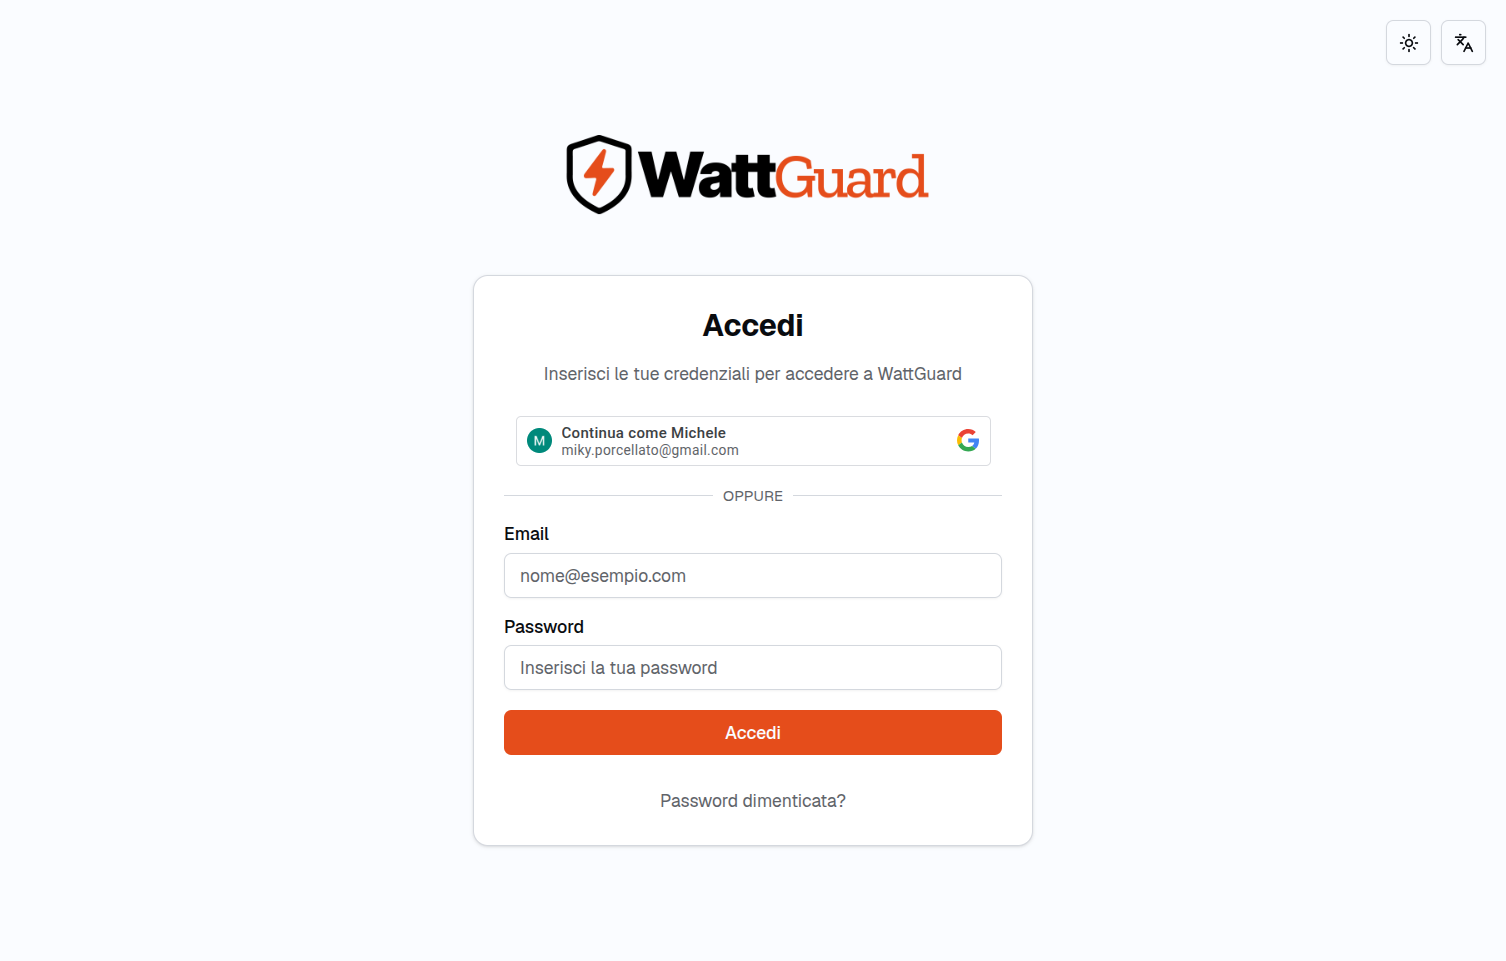
\includegraphics[width=0.75\linewidth]{../images/Frontend/login.png}
    \caption{Pagina di login}
    \label{fig:login}
\end{figure}

\begin{figure}[H]
    \centering
    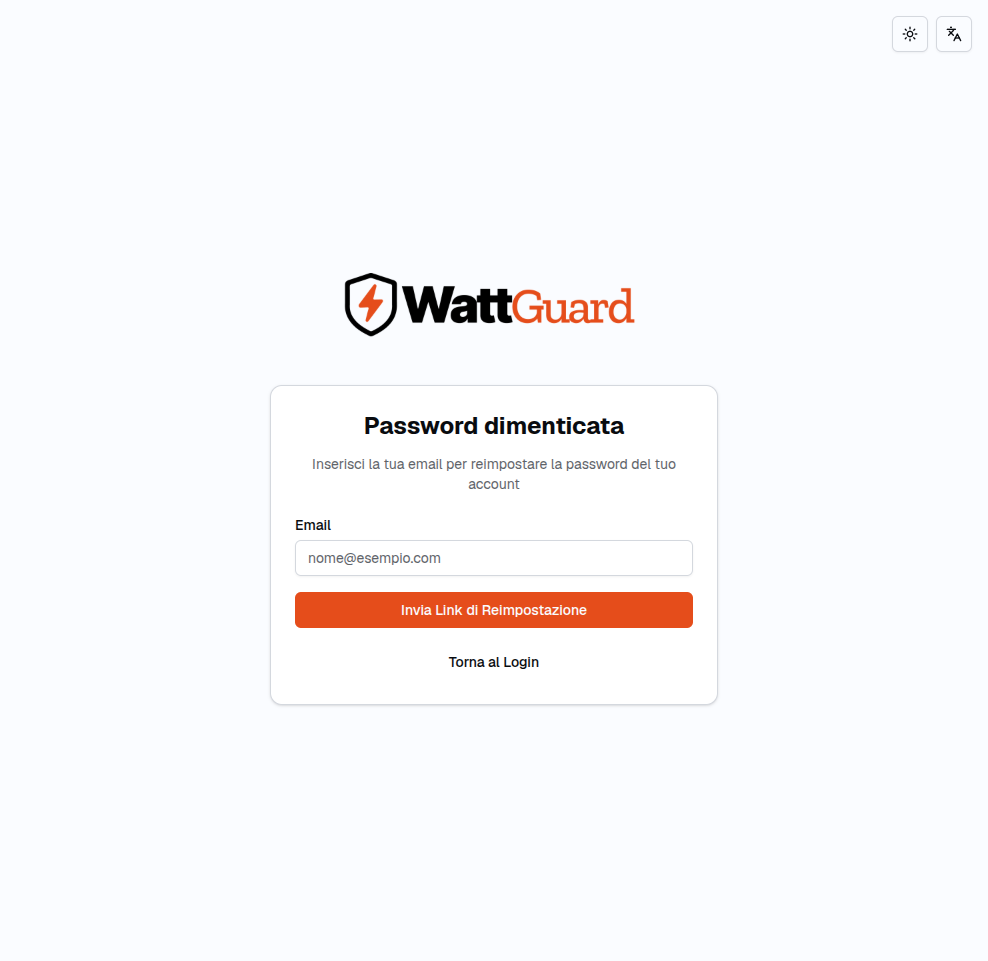
\includegraphics[width=0.5\linewidth]{../images/Frontend/forgot-password.png}
    \caption{Reset Password}
    \label{fig:reset-password}
\end{figure}


Nella \cref{fig:login} è presente la pagina principale di login, alla quale l'utente è condotto se non è attualmente loggato o il token di autenticazione JWT è scaduto.
È possibile autenticarsi sia tramite credenziali locali, inserendo e-mail e password, sia attraverso il pulsante ``Accedi con Google''

Durante la risoluzione dello stato di autenticazione viene mostrato uno \emph{spinner}.
Se l'utente viene autenticato con successo, viene reindirizzato alla dashboard principale.

Nella stessa sezione è possibile procedere con il recupero della password. (\cref{fig:reset-password})
\subsection{Accettazione Invito}

\begin{figure}[H]
    \centering
    % Prima immagine
    \begin{subfigure}[b]{0.48\textwidth}
        \centering
        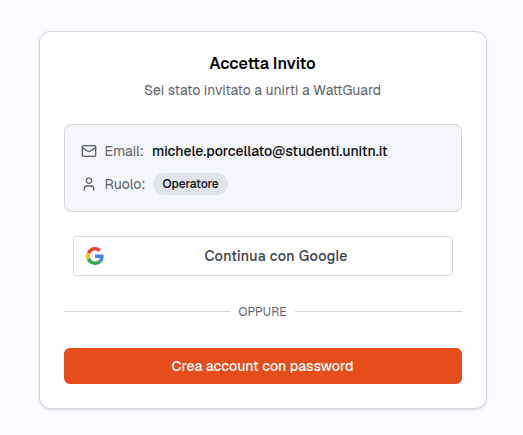
\includegraphics[width=\linewidth]{../images/Frontend/accept-invite-1.png}
        \label{fig:accept-invite-1}
    \end{subfigure}
    \hfill % Spazio orizzontale flessibile per separare le due figure
    % Seconda immagine
    \begin{subfigure}[b]{0.48\textwidth}
        \centering
        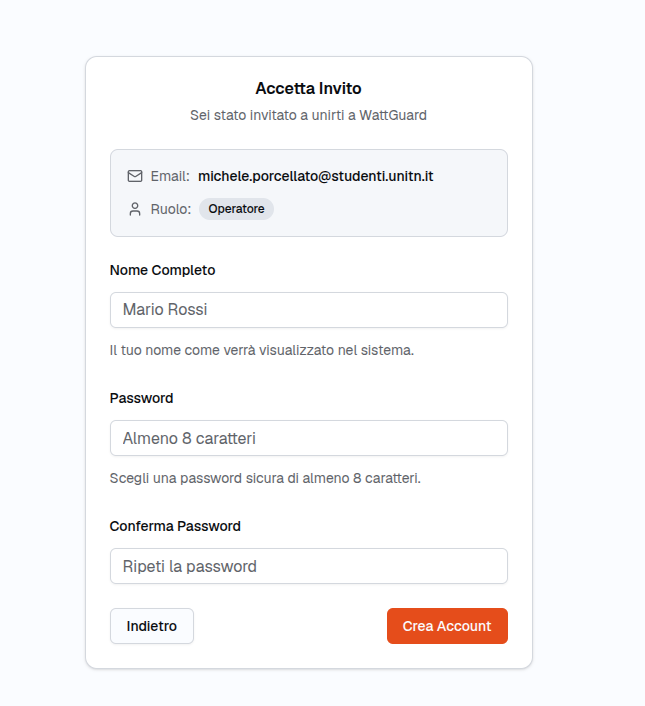
\includegraphics[width=\linewidth]{../images/Frontend/accept-invite-2.png}
        \label{fig:accept-invite-2}
    \end{subfigure}
    
    \caption{Flow di accettazione invito}
    \label{fig:accept-invite}
\end{figure}

Come illustrato nella \cref{fig:accept-invite} si illustano i passaggi necessari per accettare l'invito e completare la registrazione. Durante la registrazione è possibile procedere con il login con Google oppure creare manualmente l'utente.
Se si decide di procedere con la creazione manuale, è richiesto compilare il modulo con nome utente e password.

\subsection{Layout della dashboard}

\begin{figure}[H]
    \centering
    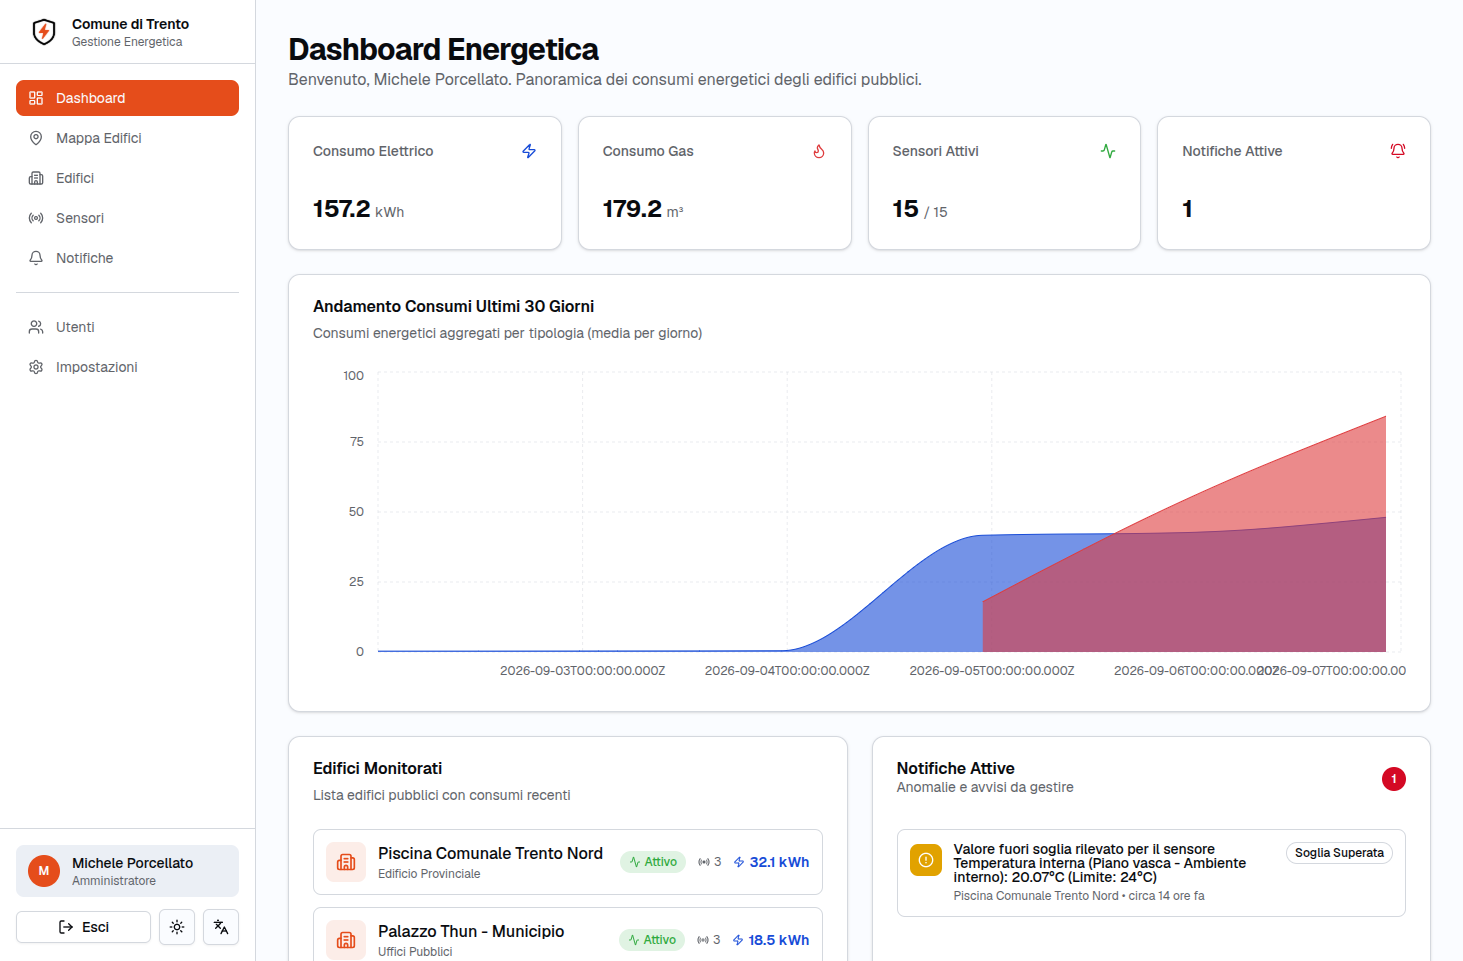
\includegraphics[width=0.80\linewidth]{../images/Frontend/dashboard.png}
    \caption{Dashboard pricnipale}
    \label{fig:dashboard}
\end{figure}

Dopo l'autenticazione l'utente si trova all'interno della dashboard. (\cref{fig:dashboard}).

Osserviamo la presenza della nav-bar a lato, la quale indica che pagina è attualmente selezionata (dashboard generare, mappa degli edifici, ricerca edifici, sensori e notifiche) e informazioni sull'utente attualmente loggato. In basso si trova il pulsante per eseguire il logout, il selettore per cambiare il tema predefinito e il selettore per cambiare la lingua del frontend (it/en/de).
Le sezioni di utenti e impostazioni sono presenti soltato per 
gli amministratori.
\newline\newline
La pagina della dashboard principale contiene i seguenti componenti:
\begin{itemize}
    \item \textbf{Informazioni complessive del sistema}: Questa sezione contiene il consumo elettrico complessivo attuale, il consumo di gas degli ultimi 30 giorni, il sensori attivi (non in manutenzione o offline) e le notifiche presenti.
    \item  \textbf{Grafico andamento dei consumi}: Il grafico mostra i consumi energetici aggregati per tipologia (celeste il consumo elettrico mentre il gas in rosso) degli ultimi 30 giorni.
    Facendo hover sul grafico compare un tooltip che mostra i dettagli del singolo punto selezionato.
    \item \textbf{Edifici Monitorati}: Mostra la lista degli edifici con i loro consumi recenti. È presente inoltre l'indicatore di quanti sensori sono presenti nell'edifico, se l'edificio è attivo o dismesso e il loro consumo istantaneo di corrente elettrica.
    \item \textbf{Notifiche attive}: Questa sezione serve per ricordare agli amministratori e agli operatori di eventuali anomalie presenti negli edifici monitorati.
\end{itemize}

I dati presenti nella dashboard vengono aggiornati automaticamente ogni 90 secondi. Questo intervallo è configurabile all'interno delle impostazioni di sistema.

\subsection{Mappa degli edifici}

\begin{figure}[H]
    \centering
    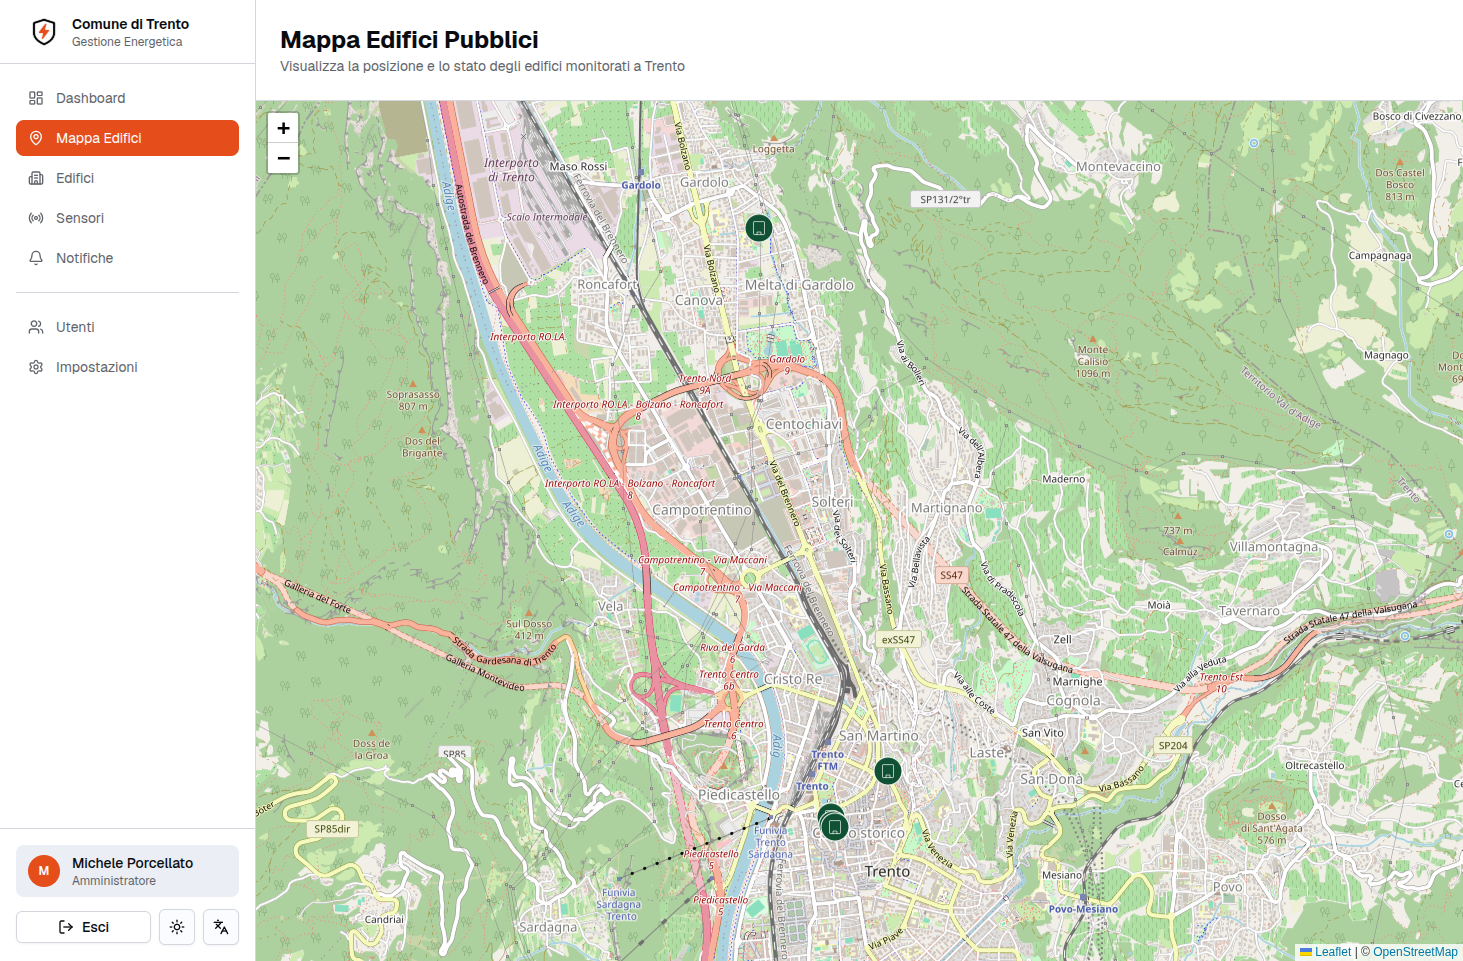
\includegraphics[width=0.80\linewidth]{../images/Frontend/map.png}
    \caption{Mappa edifici}
    \label{fig:map}
\end{figure}

Nella \cref{fig:map} si mostra la pagina contenete la disposizione geografica degli edifici monitorati su una mappa interattiva. Ogni edificio è rappresentato da un marcatore; selezionandolo, l'utente accede al dettaglio dell'edificio.
Il marcatore è verde se l'edifico risulta attivo, grigio se dismesso.

\subsection{Edifici}

\begin{figure}[H]
    \centering
    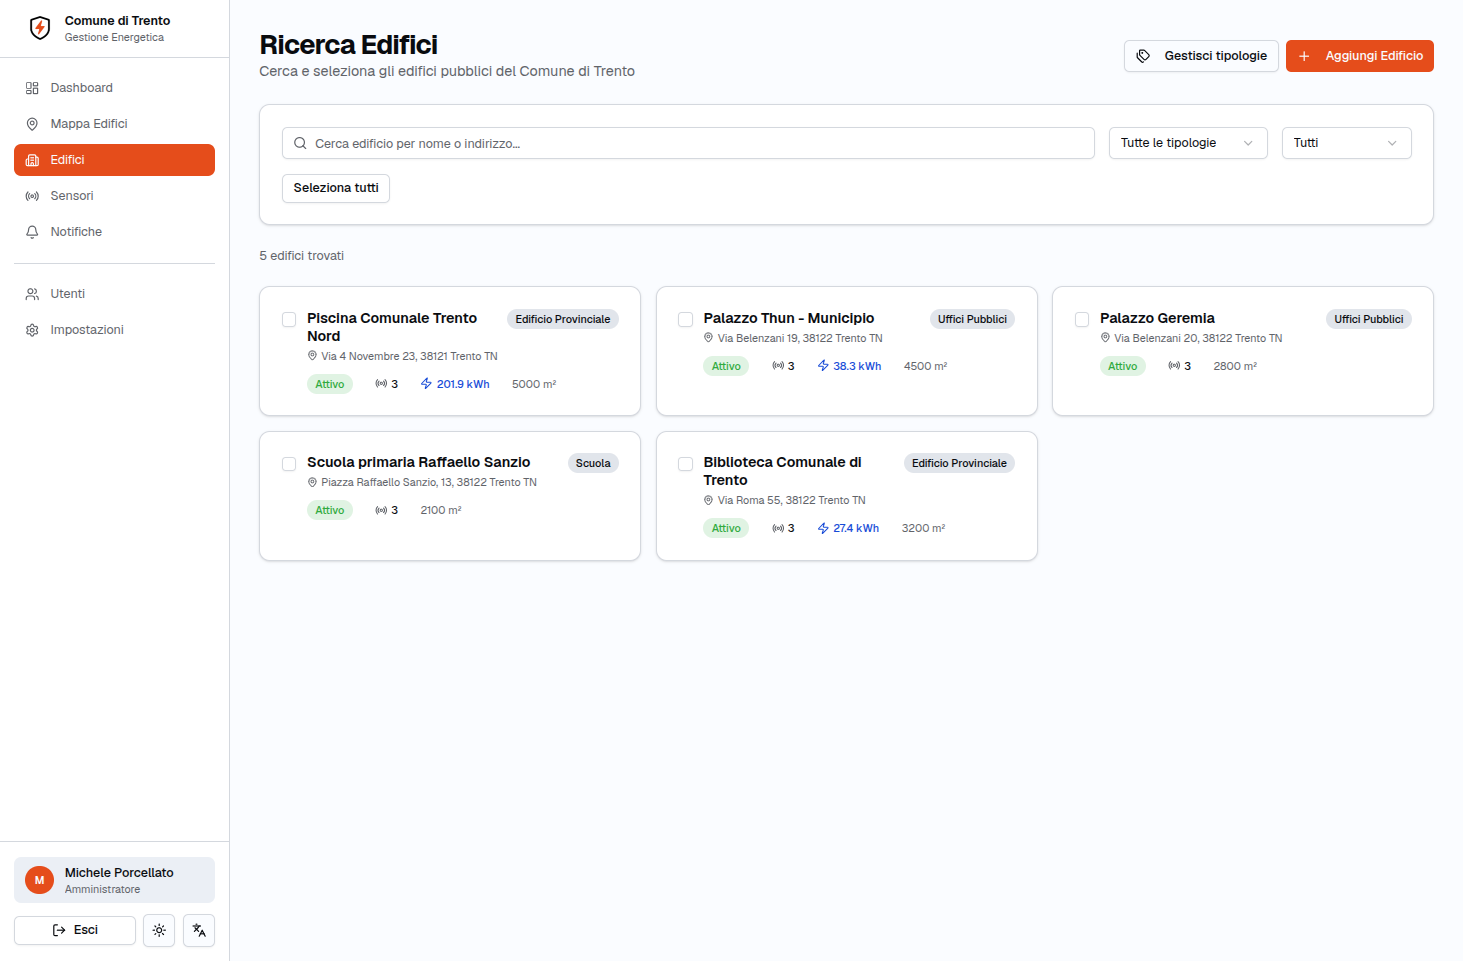
\includegraphics[width=0.80\linewidth]{../images/Frontend/buildings.png}
    \caption{Elenco edifici con ricerca}
    \label{fig:buildings}
\end{figure}

\begin{figure}[H]
    \centering
    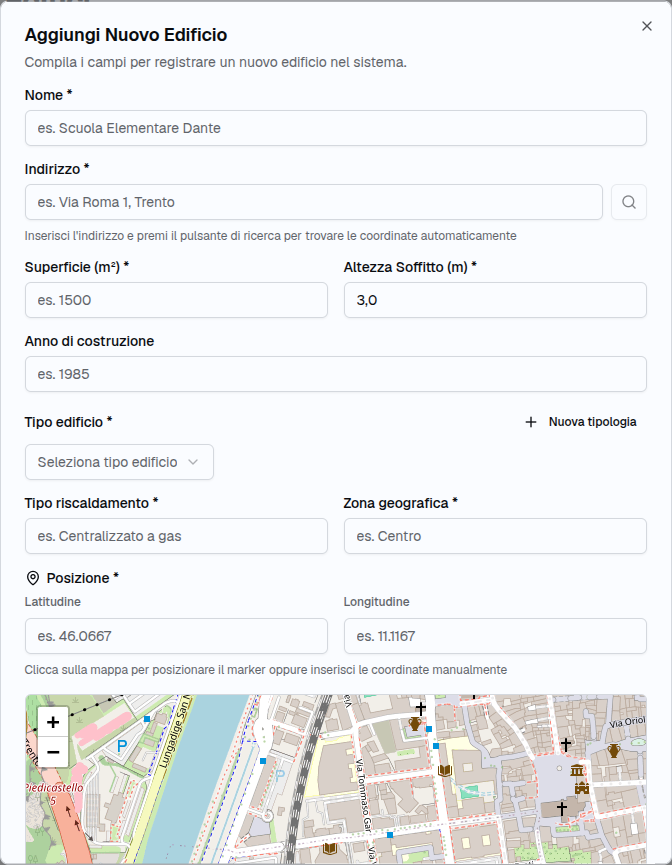
\includegraphics[width=0.5\linewidth]{../images/Frontend/create-building.png}
    \caption{Dialogo per la creazione di un nuovo edificio}
    \label{fig:create-building}
\end{figure}

In \cref{fig:buildings} è presente la sezione dedicata alla visualizzazione di tutti gli edifici.
In alto è presenta una barra di ricerca che permette di ricercare gli edifici per nome, indirizzo, zona geografica, tipologia e stato operativo.
Ogni edificio elencato presenta il nome, l'indirizzo, il numero di sensori attivi e il consumo di corrente dell'edificio.
È inoltre possibile registrare nuovi edifici, come si vede in \cref{fig:create-building}, inserendo i dati anagrafici dell'edifico e la posizione geografica (si accettato sia coordinate che indirizzo).

\subsubsection{Confronto Edifici}
\begin{figure}[H]
    \centering
    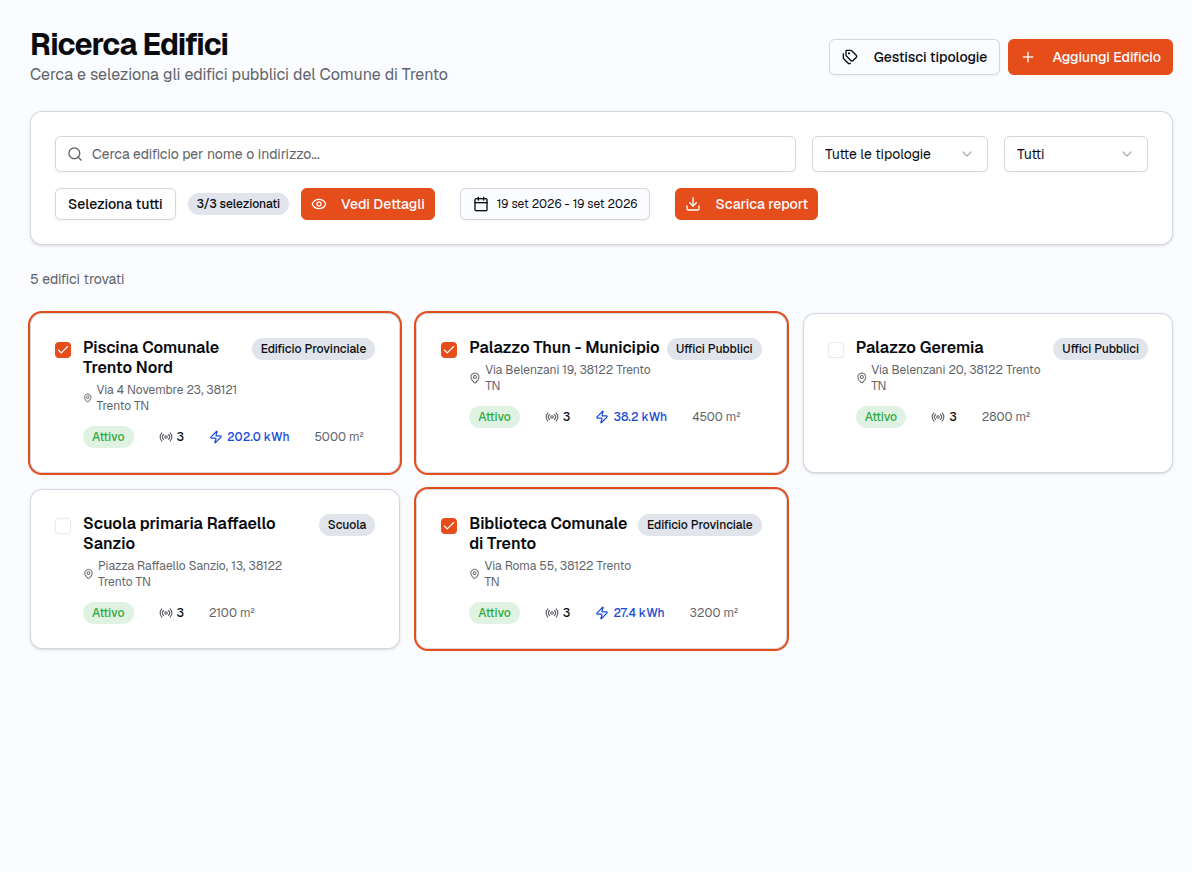
\includegraphics[width=0.8\linewidth]{../images/Frontend/compare-selected.png}
    \caption{Selezione di più edifici}
    \label{fig:building-select}
\end{figure}

\begin{figure}[H]
    \centering
    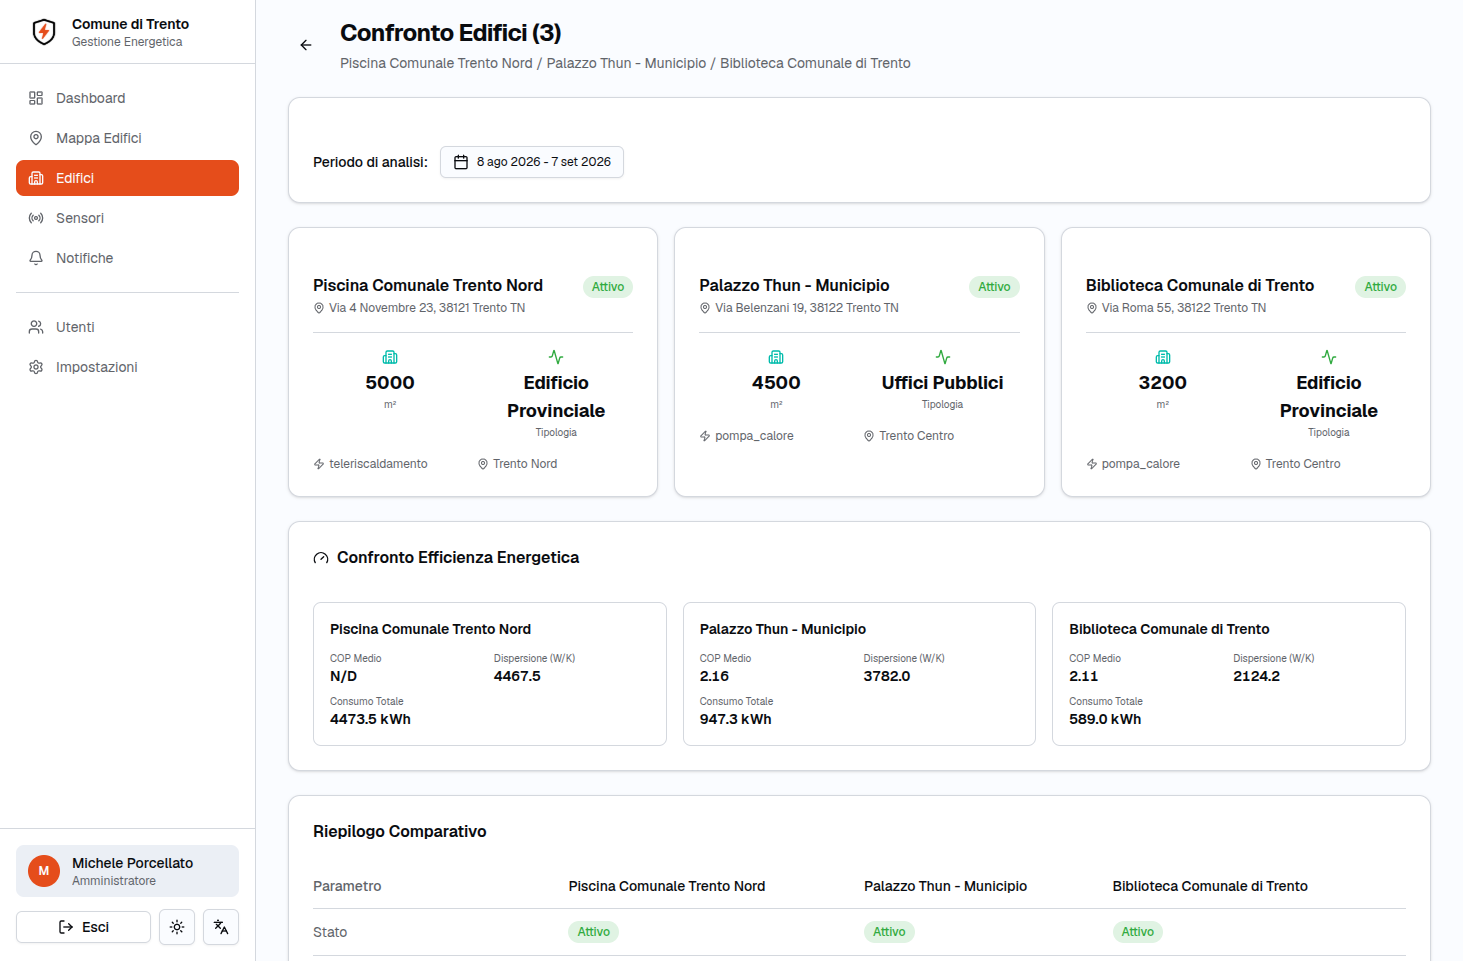
\includegraphics[width=0.8\linewidth]{../images/Frontend/compare-buildings.png}
    \caption{Pagina di comparazione}
    \label{fig:building-compare}
\end{figure}

È possibile confrontare più edifici, selezionandone al massimo 3, come si vede in \cref{fig:building-select}. Da qui è possibile scaricare sia il report dell'efficienza dei vari edifici in PDF che i valori dei vari sensori in CSV.
Cliccando su ``Vedi dettagli'' si apre la visualizzazione comparativa (\cref{fig:building-compare}).
Questa pagina mostra intuitivamente l'efficienza dei vari edifici e lo stato generale degli stessi.

\subsection{Dettaglio edificio}

\begin{figure}[H]
    \centering
    % Prima immagine
    \begin{subfigure}[b]{0.8\textwidth}
        \centering
        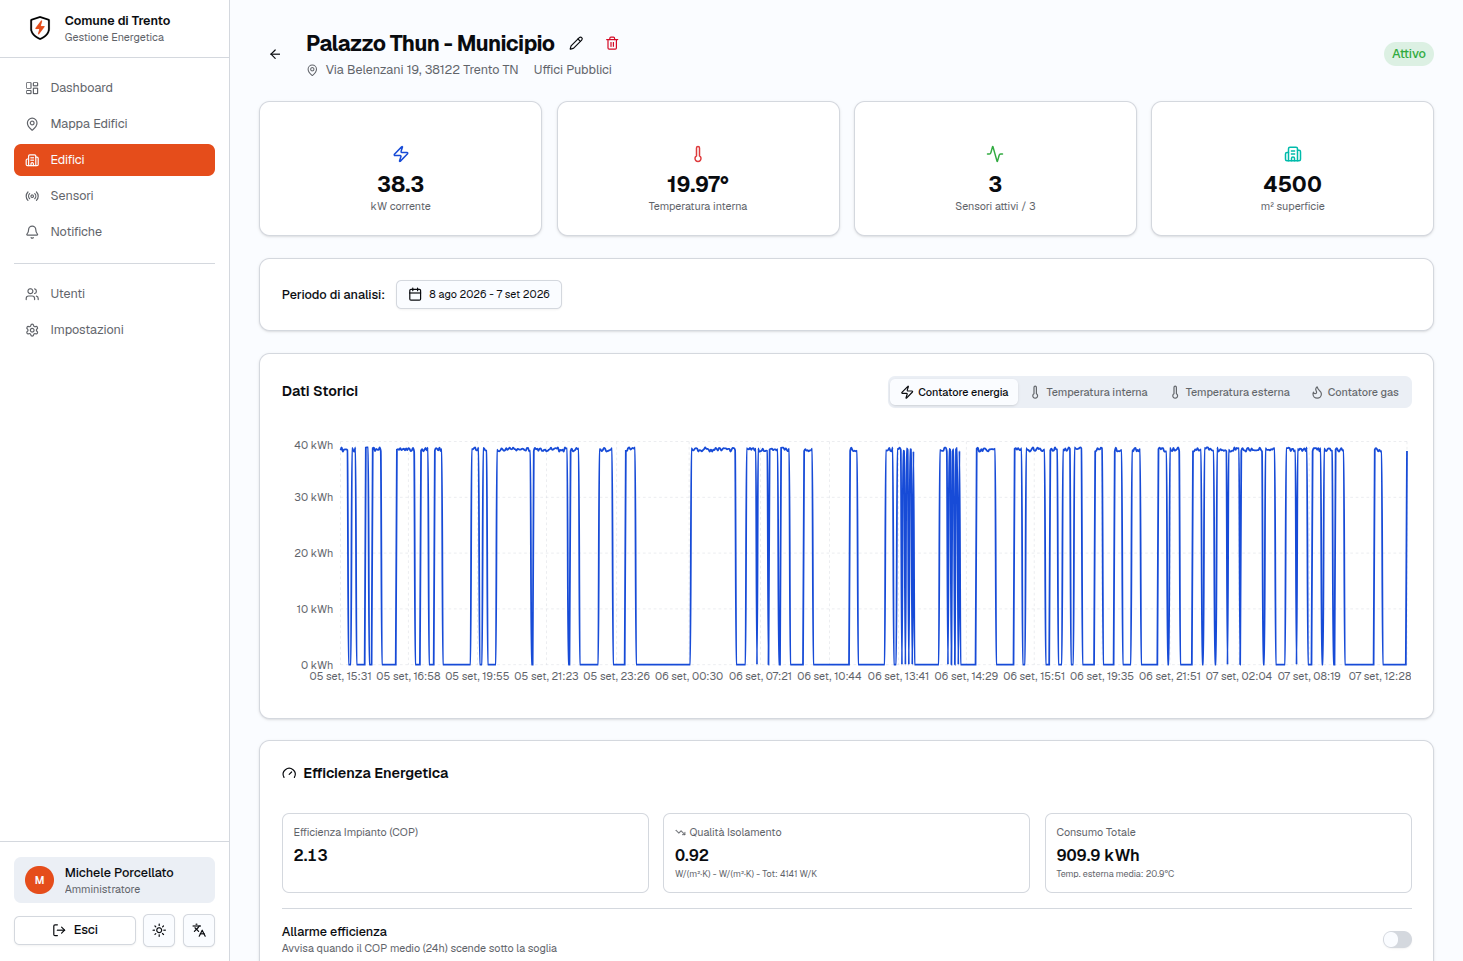
\includegraphics[width=\linewidth]{../images/Frontend/building-example-1.png}
        \label{fig:building-1}
    \end{subfigure}
    \hfill % Spazio orizzontale flessibile per separare le due figure
    % Seconda immagine
    \begin{subfigure}[b]{0.8\textwidth}
        \centering
        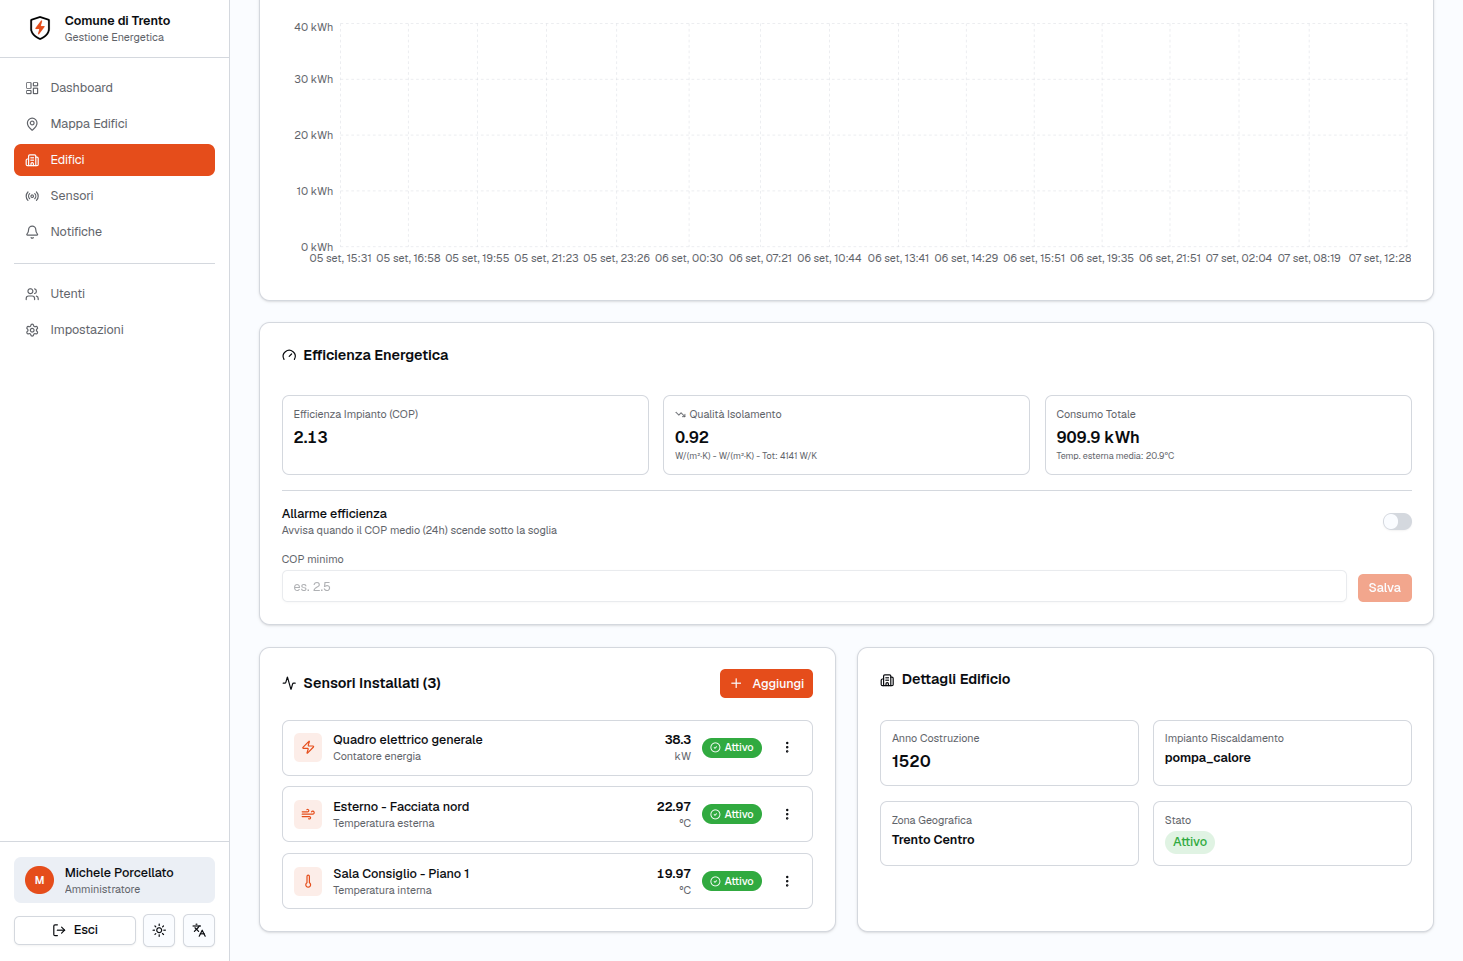
\includegraphics[width=\linewidth]{../images/Frontend/building-example-2.png}
        \label{fig:building-2}
    \end{subfigure}
    
    \caption{Pagina di dettaglio dell'edificio}
    \label{fig:building-detail}
\end{figure}

La pagina di dettaglio di un edificio riunisce i dati anagrafici e di contesto, i valori in tempo reale rilevati dai sensori, quali la temperatura interna, la temperatura esterna e il consumo istantaneo, aggiornati automaticamente, i grafici storici dei consumi e delle temperature con la possibilità di selezionare l'intervallo temporale e la grandezza di interesse, e le metriche di efficienza termica dell'edificio nel periodo selezionato, tra cui l'energia consumata, la temperatura esterna media, la dispersione termica stimata e il coefficiente di prestazione medio.

\subsection{Sensori}

\begin{figure}[H]
    \centering
    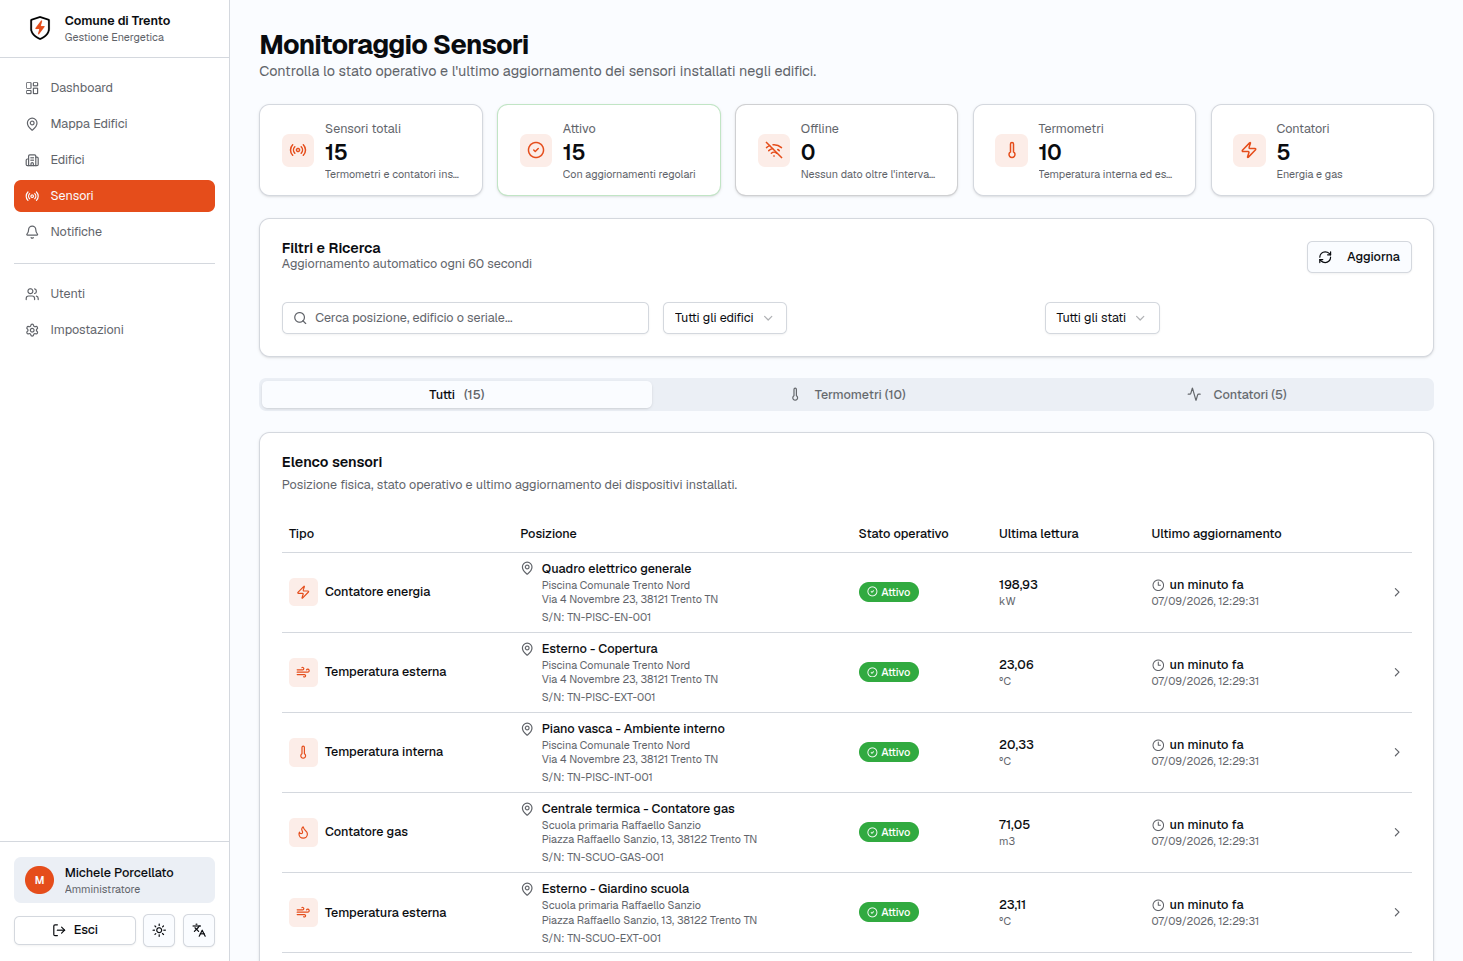
\includegraphics[width=0.8\linewidth]{../images/Frontend/sensors.png}
    \caption{Sezione sensori}
    \label{fig:sensors}
\end{figure}

\begin{figure}[H]
    \centering
    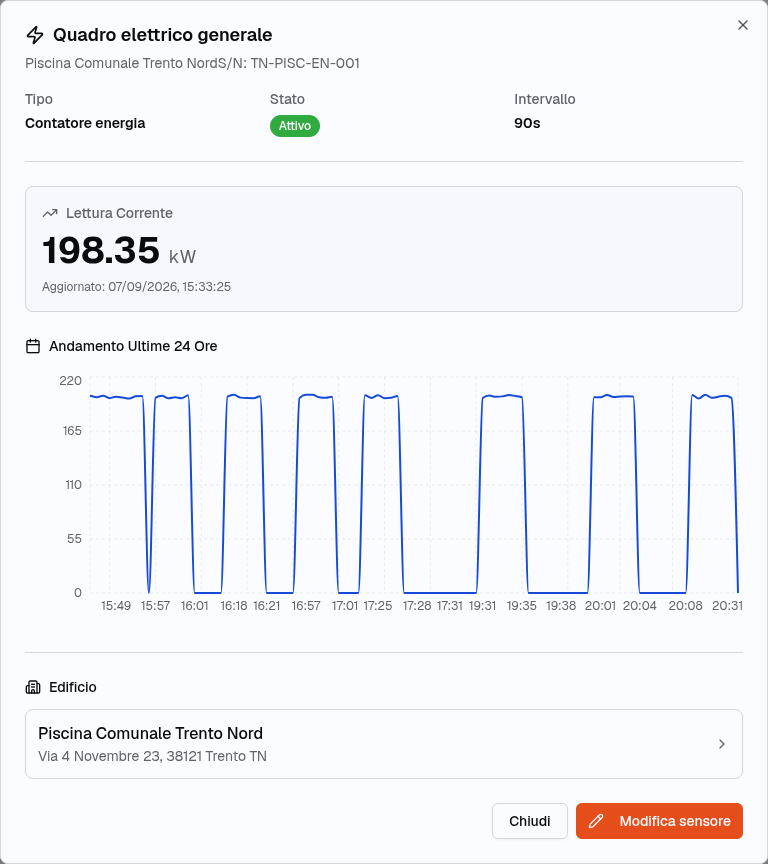
\includegraphics[height=0.5\linewidth]{../images/Frontend/sensors-detail.png}
    \caption{Dettaglio sensore}
    \label{fig:sensors-detail}
\end{figure}

In \cref{fig:sensors} è presente la sezione sensori. Essa comprende la gestione e il monitoraggio dei dispositivi installati. 
La pagina permette di registrare nuovi sensori, eseguire nuove ricerche e filtrarli per tipologia, oltre a vedre il loro stato operativo.
Cliccando sul sensore è possibile vederne i dettagli (\cref{fig:sensors-detail});
Da qui, andando su modifica sensore è possibile configurarne la tipologia, la posizione, l'intervallo di trasmissione e le soglie di allarme minima e massima.

\subsection{Allarmi}

\begin{figure}[H]
    \centering
    % Prima immagine
    \begin{subfigure}[b]{0.50\textwidth}
        \centering
        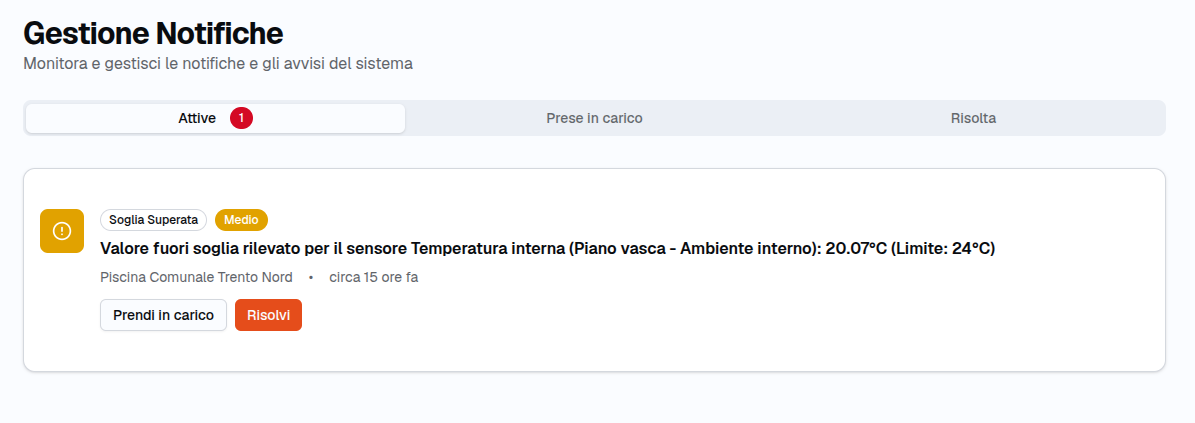
\includegraphics[width=\linewidth]{../images/Frontend/alert3.png}
        \caption{}
        \label{fig:alert-1}
    \end{subfigure}\hfill
    % Seconda immagine
    \begin{subfigure}[b]{0.50\textwidth}
        \centering
        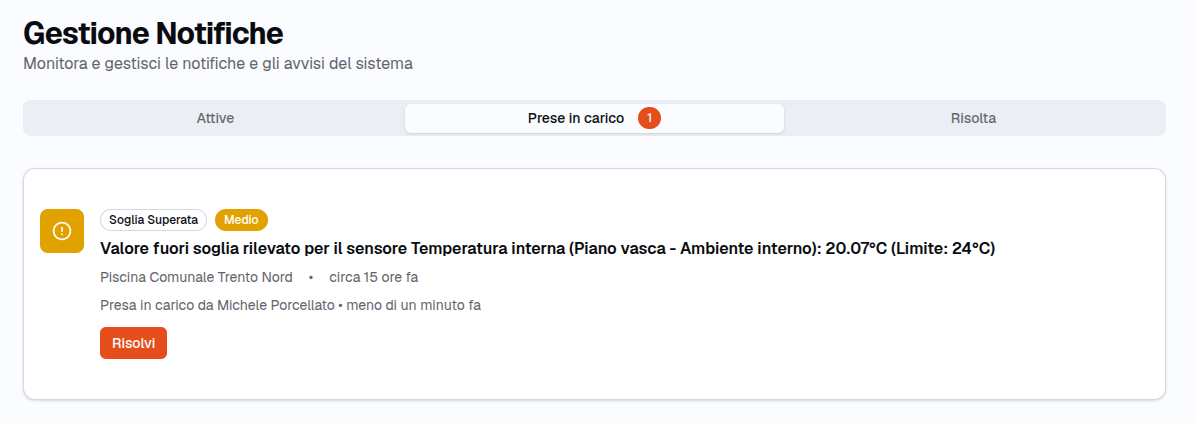
\includegraphics[width=\linewidth]{../images/Frontend/alert2.png}
        \caption{}
        \label{fig:alert-2}
    \end{subfigure}\hfill
    % Terza immagine
    \begin{subfigure}[b]{0.50\textwidth}
        \centering
        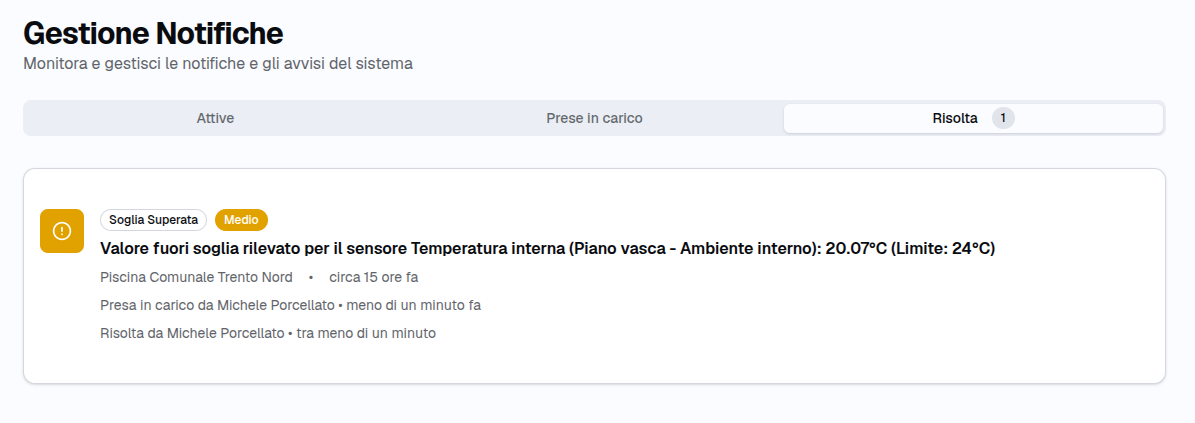
\includegraphics[width=\linewidth]{../images/Frontend/alert1.png}
        \caption{}
        \label{fig:alert-3}
    \end{subfigure}
    
    \caption{Pagina di gestione degli allarmi}
    \label{fig:alert}
\end{figure}

La pagina degli allarmi (\cref{fig:alert}) raggruppa le notifiche generate dal sistema.
Esse sono filtrabili per stato e ordinate di default per timestamp. 
Per ciascun allarme è possibile consultare i dettagli, prenderlo in carico o risolverlo.

\subsection{Amministrazione}
Le sezioni riservate agli amministratori comprendono la gestione degli utenti e le impostazioni di sistema.

\subsubsection{Utenti}
\begin{figure}[H]
    \centering
    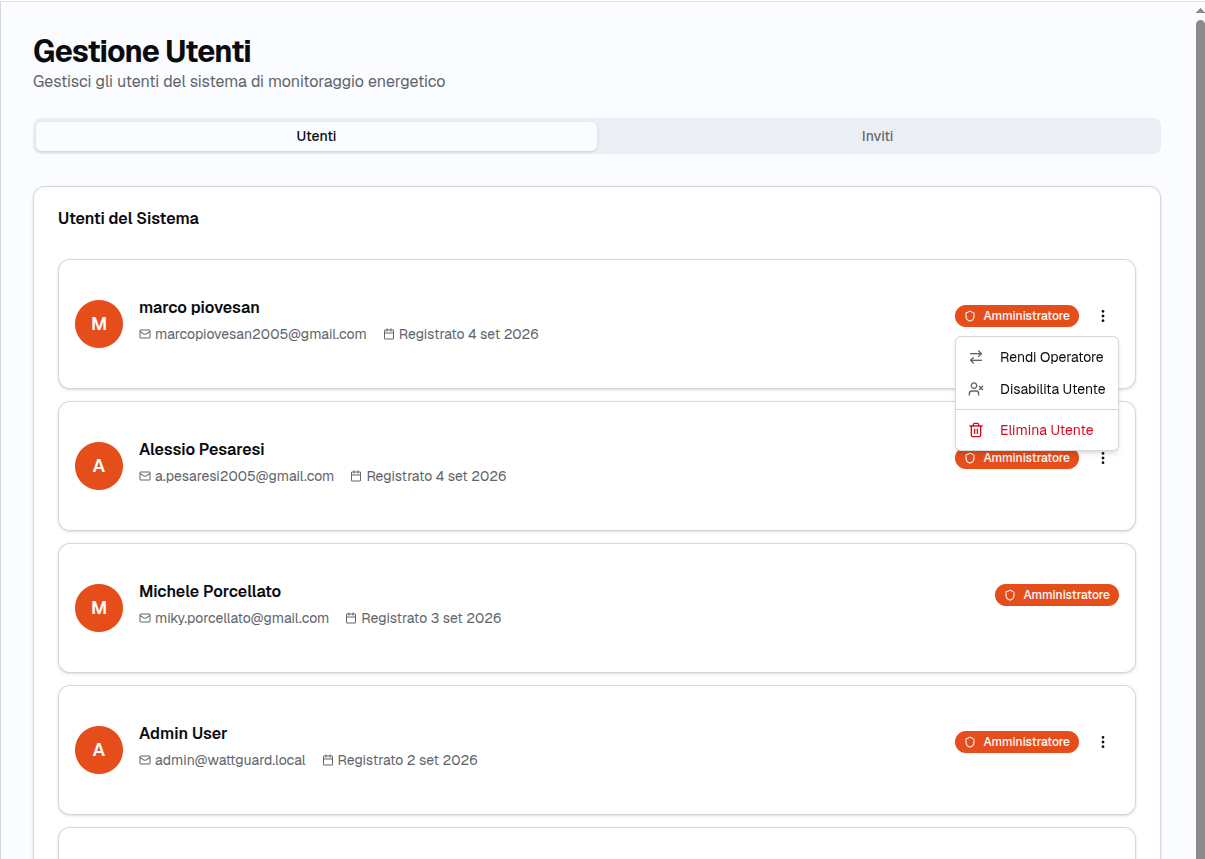
\includegraphics[width=0.8\linewidth]{../images/Frontend/users.png}
    \caption{Sezione utenti}
    \label{fig:users}
\end{figure}

\begin{figure}[H]
    \centering
    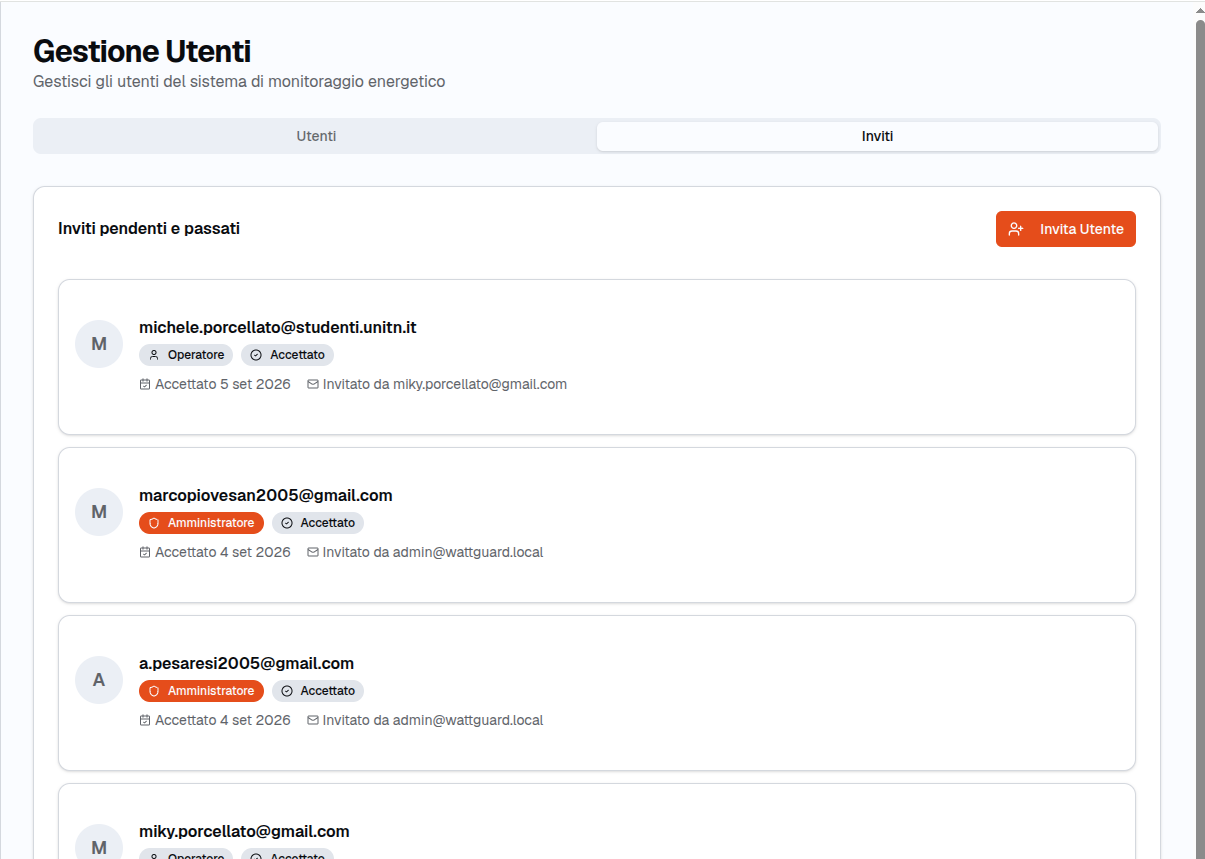
\includegraphics[width=0.8\linewidth]{../images/Frontend/invites.png}
    \caption{Sezione inviti}
    \label{fig:invites}
\end{figure}

\begin{figure}[H]
    \centering
    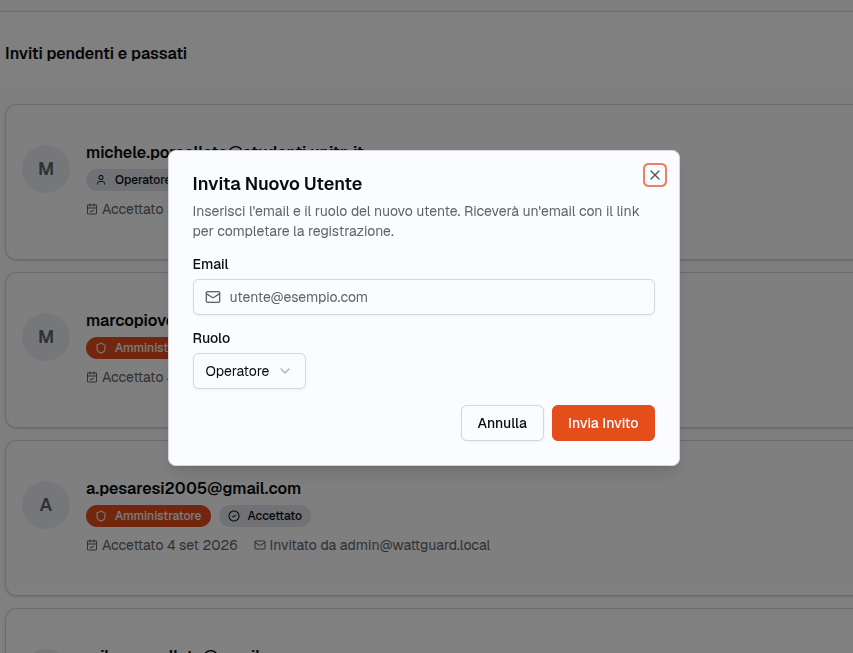
\includegraphics[width=0.5\linewidth]{../images/Frontend/invite-new-user.png}
    \caption{Dialogo invito nuovo utente}
    \label{fig:invites-dialog}
\end{figure}

Nella sezione utenti (\cref{fig:users}) è possibile controllare gli utenti presenti, cambiare il loro ruolo, disattivarli o eliminarli completamente dal sistema.

Per aggiungere nuovi utenti, è necessario recarsi nella sezione inviti (\cref{fig:invites}). Qui sono disponibili gli inviti presenti con lo stato (accettato o in attesa) e la possibilità di aggiungere nuovi utenti al sistema usando la finestra di dialogo mostrata in \cref{fig:invites-dialog}.

\subsubsection{Impostazioni di sistema}
\begin{figure}[H]
    \centering
    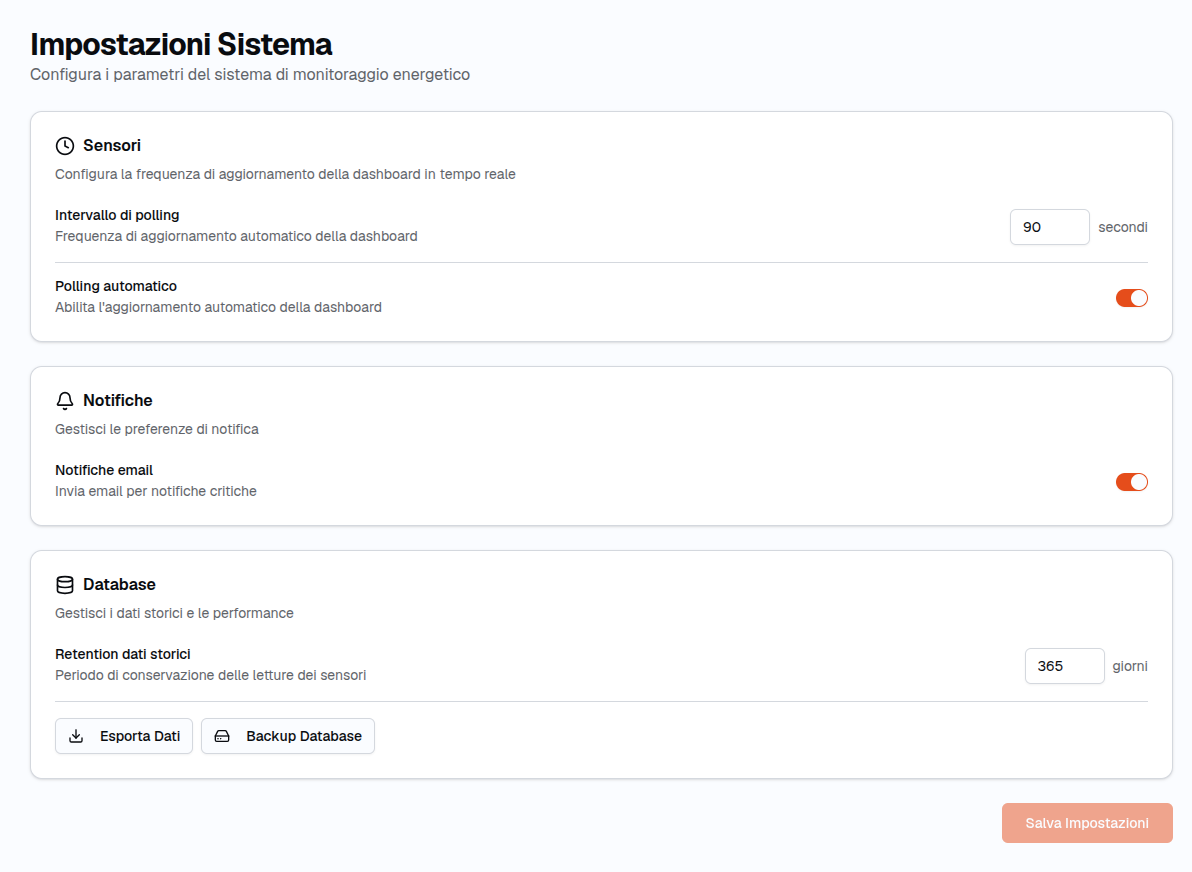
\includegraphics[width=0.8\linewidth]{../images/Frontend/settings.png}
    \caption{Impostazioni di sistema}
    \label{fig:settings}
\end{figure}

Nella pagina di impostazioni di sistema (\cref{fig:settings}) gli amministratori possono configurare l'intervallo di polling per l'aggiornamento dei valori dell'applicazione, gestire se ricevere notifiche email in caso ci siano allerte presenti e gestire i dati storici dell'applicazione (durata di conservazione, esportazione delle letture e backup del database in file JSON)

\section{Deployment}
\label{chap:deployment}

Un'istanza del backend è ospitata sulla piattaforma \emph{render.com} ed è disponibile al link \newline \href{https://wattguard.me}{wattguard.me}.
Sia backend che frontend vengono serviti presso questo indirizzo.

Il database MongoDB è invece ospitato sulla piattaforma Atlas.

\subsection{Limitazioni del deployment}
Dovute a limitazioni del piano gratuito della piattaforma Render, l'istanza dell'applicazione viene sospesa dopo 15 minuti di inattività.
Appena viene ricevuta una nuova richiesta HTTP, l'istanza torna operativa in circa un minuto (Cold Start). Di conseguenza, la prima richiesta avrà una latenza maggiore, mentre le richieste successive avranno un tempo di risposta standard.

Per superare le limitazioni imposte dalla piattaforma sono state impiegate le seguenti soluzioni: 
\begin{itemize}
    \item \textbf{Migrazione da SMTP a Resend}: Il piano gratuito di Render non permette connnesioni a server SMTP esterni. Per ovviare al problema si è impiegata il servizio  \textbf{Resend} e la sua libreria. Questo servizio, anch'esso gratuito, permette di mandare mail tramite richieste HTTP, aggirando le restrizioni imposte.
    \item \textbf{Dominio certificato per le mail}: Per usufruire dei servizi di Resend è necessario possedere un dominio. Ci siamo affidati a \textbf{Namecheap} registrando il dominio \texttt{wattguard.me} e configurando i record DNS richiesti (record TXT)
    \item \textbf{Simulatore in-process} Dato che non disponiamo né di un broker MQTT esterno, né di ulteriori risorse di calcolo per simulare una topologia di sensori realistica, tutte le misurazioni dei sensori sono create con un simulatore interno all'applicazione. Questa scelta comporta un limite: l'eventuale sospensione dell'istanza di Render comporta l'interruzione anche del simulatore, facendo apparire i sensori offline. 
\end{itemize}

\subsection{Configurazione CI/CD}
La configurazione CI/CD basata su GitHub Action esegue le verifiche automatiche del codice ad ogni push sui rami \texttt{main} e \texttt{develop}.
Le verifiche comprendono:
\begin{itemize}
    \item \texttt{bun run check} Controllo dei tipi statici da parte del compilatore TypeScript;
    \item \texttt{bun run lint} Analisi statica del codice (linting) fornita da \texttt{oxlint};
    \item \texttt{bun run test} Esecuzione dei test unitari e di integrazione;
    \item  \texttt{bun run build} Generazione dei file di bundle e degli asset finali.
\end{itemize}
Nel caso le verifiche abbiano successo e ci si trova nel ramo \texttt{main} viene anche eseguito il deploy su Render.

\subsection{Credenziali e accesso docenti}
Per accedere al deploy dell'applicazione è possibile utilizzare i seguenti account:
\begin{center}
\textbf{Utente amministratore}
    \begin{itemize}
        \item \textbf{Email}: \texttt{admin@wattguard.local}
        \item \textbf{Password}: \texttt{admin123}
    \end{itemize}
\textbf{Utente operatore}
    \begin{itemize}
        \item \textbf{Email}: \texttt{operator@wattguard.local}
        \item \textbf{Password}: \texttt{operator456}
    \end{itemize}
\end{center}
\vspace{1cm}
In caso di problemi con il deployment contattare:
\begin{itemize}
    \item \href{mailto:michele.porcellato@studenti.unitn.it}{michele.porcellato@studenti.unitn.it}
    \item \href{mailto:marco.piovesan-2@studenti.unitn.it}{marco.piovesan-2@studenti.unitn.it}
    \item \href{mailto:alessio.pesaresi@studenti.unitn.it}{alessio.pesaresi@studenti.unitn.it}
\end{itemize}
\end{document}